\documentclass[twoside]{book}

% Packages required by doxygen
\usepackage{fixltx2e}
\usepackage{calc}
\usepackage{doxygen}
\usepackage[export]{adjustbox} % also loads graphicx
\usepackage{graphicx}
\usepackage[utf8]{inputenc}
\usepackage{makeidx}
\usepackage{multicol}
\usepackage{multirow}
\PassOptionsToPackage{warn}{textcomp}
\usepackage{textcomp}
\usepackage[nointegrals]{wasysym}
\usepackage[table]{xcolor}

% Font selection
\usepackage[T1]{fontenc}
\usepackage[scaled=.90]{helvet}
\usepackage{courier}
\usepackage{amssymb}
\usepackage{sectsty}
\renewcommand{\familydefault}{\sfdefault}
\allsectionsfont{%
  \fontseries{bc}\selectfont%
  \color{darkgray}%
}
\renewcommand{\DoxyLabelFont}{%
  \fontseries{bc}\selectfont%
  \color{darkgray}%
}
\newcommand{\+}{\discretionary{\mbox{\scriptsize$\hookleftarrow$}}{}{}}

% Page & text layout
\usepackage{geometry}
\geometry{%
  a4paper,%
  top=2.5cm,%
  bottom=2.5cm,%
  left=2.5cm,%
  right=2.5cm%
}
\tolerance=750
\hfuzz=15pt
\hbadness=750
\setlength{\emergencystretch}{15pt}
\setlength{\parindent}{0cm}
\setlength{\parskip}{3ex plus 2ex minus 2ex}
\makeatletter
\renewcommand{\paragraph}{%
  \@startsection{paragraph}{4}{0ex}{-1.0ex}{1.0ex}{%
    \normalfont\normalsize\bfseries\SS@parafont%
  }%
}
\renewcommand{\subparagraph}{%
  \@startsection{subparagraph}{5}{0ex}{-1.0ex}{1.0ex}{%
    \normalfont\normalsize\bfseries\SS@subparafont%
  }%
}
\makeatother

% Headers & footers
\usepackage{fancyhdr}
\pagestyle{fancyplain}
\fancyhead[LE]{\fancyplain{}{\bfseries\thepage}}
\fancyhead[CE]{\fancyplain{}{}}
\fancyhead[RE]{\fancyplain{}{\bfseries\leftmark}}
\fancyhead[LO]{\fancyplain{}{\bfseries\rightmark}}
\fancyhead[CO]{\fancyplain{}{}}
\fancyhead[RO]{\fancyplain{}{\bfseries\thepage}}
\fancyfoot[LE]{\fancyplain{}{}}
\fancyfoot[CE]{\fancyplain{}{}}
\fancyfoot[RE]{\fancyplain{}{\bfseries\scriptsize Generated by Doxygen }}
\fancyfoot[LO]{\fancyplain{}{\bfseries\scriptsize Generated by Doxygen }}
\fancyfoot[CO]{\fancyplain{}{}}
\fancyfoot[RO]{\fancyplain{}{}}
\renewcommand{\footrulewidth}{0.4pt}
\renewcommand{\chaptermark}[1]{%
  \markboth{#1}{}%
}
\renewcommand{\sectionmark}[1]{%
  \markright{\thesection\ #1}%
}

% Indices & bibliography
\usepackage{natbib}
\usepackage[titles]{tocloft}
\setcounter{tocdepth}{3}
\setcounter{secnumdepth}{5}
\makeindex

% Hyperlinks (required, but should be loaded last)
\usepackage{ifpdf}
\ifpdf
  \usepackage[pdftex,pagebackref=true]{hyperref}
\else
  \usepackage[ps2pdf,pagebackref=true]{hyperref}
\fi
\hypersetup{%
  colorlinks=true,%
  linkcolor=blue,%
  citecolor=blue,%
  unicode%
}

% Custom commands
\newcommand{\clearemptydoublepage}{%
  \newpage{\pagestyle{empty}\cleardoublepage}%
}

\usepackage{caption}
\captionsetup{labelsep=space,justification=centering,font={bf},singlelinecheck=off,skip=4pt,position=top}

%===== C O N T E N T S =====

\begin{document}

% Titlepage & ToC
\hypersetup{pageanchor=false,
             bookmarksnumbered=true,
             pdfencoding=unicode
            }
\pagenumbering{roman}
\begin{titlepage}
\vspace*{7cm}
\begin{center}%
{\Large Final Project }\\
\vspace*{1cm}
{\large Generated by Doxygen 1.8.11}\\
\end{center}
\end{titlepage}
\clearemptydoublepage
\tableofcontents
\clearemptydoublepage
\pagenumbering{arabic}
\hypersetup{pageanchor=true}

%--- Begin generated contents ---
\chapter{C\+S5201\+\_\+final\+Proj}
\label{md_README}
\hypertarget{md_README}{}
\input{md_README}
\chapter{Hierarchical Index}
\section{Class Hierarchy}
This inheritance list is sorted roughly, but not completely, alphabetically\+:\begin{DoxyCompactList}
\item \contentsline{section}{Compare$<$ T $>$}{\pageref{classCompare}}{}
\item \contentsline{section}{deep\+Dec$<$ T $>$}{\pageref{classdeepDec}}{}
\item \contentsline{section}{gauss\+\_\+seidel$<$ T $>$}{\pageref{classgauss__seidel}}{}
\item \contentsline{section}{Matrix$<$ T $>$}{\pageref{classMatrix}}{}
\begin{DoxyCompactList}
\item \contentsline{section}{sym\+Matrix$<$ T $>$}{\pageref{classsymMatrix}}{}
\end{DoxyCompactList}
\item \contentsline{section}{mesh$<$ T $>$}{\pageref{classmesh}}{}
\item \contentsline{section}{My\+Array$<$ T $>$}{\pageref{classMyArray}}{}
\item \contentsline{section}{My\+Array$<$ My\+Array$<$ T $>$ $>$}{\pageref{classMyArray}}{}
\end{DoxyCompactList}

\chapter{Class Index}
\section{Class List}
Here are the classes, structs, unions and interfaces with brief descriptions\+:\begin{DoxyCompactList}
\item\contentsline{section}{\hyperlink{classCompare}{Compare$<$ T $>$} }{\pageref{classCompare}}{}
\item\contentsline{section}{\hyperlink{classdeepDec}{deep\+Dec$<$ T $>$} }{\pageref{classdeepDec}}{}
\item\contentsline{section}{\hyperlink{classgauss__seidel}{gauss\+\_\+seidel$<$ T $>$} }{\pageref{classgauss__seidel}}{}
\item\contentsline{section}{\hyperlink{classMatrix}{Matrix$<$ T $>$} }{\pageref{classMatrix}}{}
\item\contentsline{section}{\hyperlink{classmesh}{mesh$<$ T $>$} }{\pageref{classmesh}}{}
\item\contentsline{section}{\hyperlink{classMyArray}{My\+Array$<$ T $>$} }{\pageref{classMyArray}}{}
\item\contentsline{section}{\hyperlink{classsymMatrix}{sym\+Matrix$<$ T $>$} }{\pageref{classsymMatrix}}{}
\end{DoxyCompactList}

\chapter{File Index}
\section{File List}
Here is a list of all documented files with brief descriptions\+:\begin{DoxyCompactList}
\item\contentsline{section}{\hyperlink{deepdec_8h}{deepdec.\+h} }{\pageref{deepdec_8h}}{}
\item\contentsline{section}{{\bfseries deepdec.\+hpp} }{\pageref{deepdec_8hpp}}{}
\item\contentsline{section}{{\bfseries functions.\+h} }{\pageref{functions_8h}}{}
\item\contentsline{section}{\hyperlink{gauss__seidel_8h}{gauss\+\_\+seidel.\+h} }{\pageref{gauss__seidel_8h}}{}
\item\contentsline{section}{{\bfseries gauss\+\_\+seidel.\+hpp} }{\pageref{gauss__seidel_8hpp}}{}
\item\contentsline{section}{\hyperlink{matrix_8h}{matrix.\+h} }{\pageref{matrix_8h}}{}
\item\contentsline{section}{{\bfseries matrix.\+hpp} }{\pageref{matrix_8hpp}}{}
\item\contentsline{section}{\hyperlink{mesh_8h}{mesh.\+h} }{\pageref{mesh_8h}}{}
\item\contentsline{section}{{\bfseries mesh.\+hpp} }{\pageref{mesh_8hpp}}{}
\item\contentsline{section}{\hyperlink{myArray_8h}{my\+Array.\+h} }{\pageref{myArray_8h}}{}
\item\contentsline{section}{{\bfseries my\+Array.\+hpp} }{\pageref{myArray_8hpp}}{}
\item\contentsline{section}{\hyperlink{symMatrix_8h}{sym\+Matrix.\+h} }{\pageref{symMatrix_8h}}{}
\item\contentsline{section}{{\bfseries sym\+Matrix.\+hpp} }{\pageref{symMatrix_8hpp}}{}
\end{DoxyCompactList}

\chapter{Class Documentation}
\hypertarget{classCompare}{}\section{Compare$<$ T $>$ Class Template Reference}
\label{classCompare}\index{Compare$<$ T $>$@{Compare$<$ T $>$}}


{\ttfamily \#include $<$matrix.\+h$>$}

\subsection*{Public Member Functions}
\begin{DoxyCompactItemize}
\item 
bool \hyperlink{classCompare_a6024147b908ca76c18ef56bc59f59147}{operator()} (const tuple$<$ T, int $>$ lhs, const tuple$<$ T, int $>$ rhs) const 
\end{DoxyCompactItemize}


\subsection{Detailed Description}
\subsubsection*{template$<$typename T$>$\\*
class Compare$<$ T $>$}

The compare Class. 

\subsection{Member Function Documentation}
\index{Compare@{Compare}!operator()@{operator()}}
\index{operator()@{operator()}!Compare@{Compare}}
\subsubsection[{\texorpdfstring{operator()(const tuple$<$ T, int $>$ lhs, const tuple$<$ T, int $>$ rhs) const }{operator()(const tuple< T, int > lhs, const tuple< T, int > rhs) const }}]{\setlength{\rightskip}{0pt plus 5cm}template$<$typename T $>$ bool {\bf Compare}$<$ T $>$\+::operator() (
\begin{DoxyParamCaption}
\item[{const tuple$<$ T, int $>$}]{lhs, }
\item[{const tuple$<$ T, int $>$}]{rhs}
\end{DoxyParamCaption}
) const\hspace{0.3cm}{\ttfamily [inline]}}\hypertarget{classCompare_a6024147b908ca76c18ef56bc59f59147}{}\label{classCompare_a6024147b908ca76c18ef56bc59f59147}
The () Operator returns true if lhs $<$ rhs \begin{DoxyPrecond}{Precondition}
\textquotesingle{}$<$\textquotesingle{} operator defind for T! 
\end{DoxyPrecond}
\begin{DoxyPostcond}{Postcondition}
none 
\end{DoxyPostcond}


The documentation for this class was generated from the following file\+:\begin{DoxyCompactItemize}
\item 
\hyperlink{matrix_8h}{matrix.\+h}\end{DoxyCompactItemize}

\hypertarget{classdeepDec}{}\section{deep\+Dec$<$ T $>$ Class Template Reference}
\label{classdeepDec}\index{deep\+Dec$<$ T $>$@{deep\+Dec$<$ T $>$}}


{\ttfamily \#include $<$deepdec.\+h$>$}

\subsection*{Public Member Functions}
\begin{DoxyCompactItemize}
\item 
\hyperlink{classMyArray}{My\+Array}$<$ T $>$ \hyperlink{classdeepDec_a4984e6083a3b5ab7eb22e0576d6d4b8b}{operator()} (const \hyperlink{classsymMatrix}{sym\+Matrix}$<$ T $>$ mat, const \hyperlink{classMyArray}{My\+Array}$<$ T $>$ arr) const 
\end{DoxyCompactItemize}


\subsection{Detailed Description}
\subsubsection*{template$<$typename T$>$\\*
class deep\+Dec$<$ T $>$}

the steepest descent calculation class 

\subsection{Member Function Documentation}
\index{deep\+Dec@{deep\+Dec}!operator()@{operator()}}
\index{operator()@{operator()}!deep\+Dec@{deep\+Dec}}
\subsubsection[{\texorpdfstring{operator()(const sym\+Matrix$<$ T $>$ mat, const My\+Array$<$ T $>$ arr) const }{operator()(const symMatrix< T > mat, const MyArray< T > arr) const }}]{\setlength{\rightskip}{0pt plus 5cm}template$<$typename T $>$ {\bf My\+Array}$<$ T $>$ {\bf deep\+Dec}$<$ T $>$\+::operator() (
\begin{DoxyParamCaption}
\item[{const {\bf sym\+Matrix}$<$ T $>$}]{mat, }
\item[{const {\bf My\+Array}$<$ T $>$}]{arr}
\end{DoxyParamCaption}
) const}\hypertarget{classdeepDec_a4984e6083a3b5ab7eb22e0576d6d4b8b}{}\label{classdeepDec_a4984e6083a3b5ab7eb22e0576d6d4b8b}
Operator () calculator! \begin{DoxyPrecond}{Precondition}
T must have the\+: \char`\"{}$\ast$\char`\"{} \char`\"{}/\char`\"{} \char`\"{}-\/\char`\"{} binary operators defiend for it 
\end{DoxyPrecond}
\begin{DoxyPostcond}{Postcondition}
a New Array$<$\+T$>$ is born 
\end{DoxyPostcond}
\begin{DoxyReturn}{Returns}
steepest descent result for Ax=b. Where A is the Symetric \hyperlink{classMatrix}{Matrix} and b is the Array 
\end{DoxyReturn}


The documentation for this class was generated from the following files\+:\begin{DoxyCompactItemize}
\item 
\hyperlink{deepdec_8h}{deepdec.\+h}\item 
deepdec.\+hpp\end{DoxyCompactItemize}

\hypertarget{classgauss__seidel}{}\section{gauss\+\_\+seidel$<$ T $>$ Class Template Reference}
\label{classgauss__seidel}\index{gauss\+\_\+seidel$<$ T $>$@{gauss\+\_\+seidel$<$ T $>$}}


{\ttfamily \#include $<$gauss\+\_\+seidel.\+h$>$}

\subsection*{Public Member Functions}
\begin{DoxyCompactItemize}
\item 
\hyperlink{classMyArray}{My\+Array}$<$ T $>$ \hyperlink{classgauss__seidel_a09ebc3c2c01756a862ef6c27a513ee78}{operator()} (const \hyperlink{classsymMatrix}{sym\+Matrix}$<$ T $>$ \&arr, const \hyperlink{classMyArray}{My\+Array}$<$ T $>$ \&vec) const 
\end{DoxyCompactItemize}


\subsection{Detailed Description}
\subsubsection*{template$<$typename T$>$\\*
class gauss\+\_\+seidel$<$ T $>$}

the Gauss-\/\+Seidel calculation class 

\subsection{Member Function Documentation}
\index{gauss\+\_\+seidel@{gauss\+\_\+seidel}!operator()@{operator()}}
\index{operator()@{operator()}!gauss\+\_\+seidel@{gauss\+\_\+seidel}}
\subsubsection[{\texorpdfstring{operator()(const sym\+Matrix$<$ T $>$ \&arr, const My\+Array$<$ T $>$ \&vec) const }{operator()(const symMatrix< T > &arr, const MyArray< T > &vec) const }}]{\setlength{\rightskip}{0pt plus 5cm}template$<$typename T $>$ {\bf My\+Array}$<$ T $>$ {\bf gauss\+\_\+seidel}$<$ T $>$\+::operator() (
\begin{DoxyParamCaption}
\item[{const {\bf sym\+Matrix}$<$ T $>$ \&}]{arr, }
\item[{const {\bf My\+Array}$<$ T $>$ \&}]{vec}
\end{DoxyParamCaption}
) const}\hypertarget{classgauss__seidel_a09ebc3c2c01756a862ef6c27a513ee78}{}\label{classgauss__seidel_a09ebc3c2c01756a862ef6c27a513ee78}
Operator () calculator! \begin{DoxyPrecond}{Precondition}
T must have the\+: \char`\"{}$\ast$\char`\"{} \char`\"{}/\char`\"{} \char`\"{}+=\char`\"{} binary operators defiend for it 
\end{DoxyPrecond}
\begin{DoxyPostcond}{Postcondition}
a New Array$<$\+T$>$ is born 
\end{DoxyPostcond}
\begin{DoxyReturn}{Returns}
Gauss-\/\+Seidel result for Ax=b. Where A is the Symetric \hyperlink{classMatrix}{Matrix} and b is the Array 
\end{DoxyReturn}


The documentation for this class was generated from the following files\+:\begin{DoxyCompactItemize}
\item 
\hyperlink{gauss__seidel_8h}{gauss\+\_\+seidel.\+h}\item 
gauss\+\_\+seidel.\+hpp\end{DoxyCompactItemize}

\hypertarget{classMatrix}{}\section{Matrix$<$ T $>$ Class Template Reference}
\label{classMatrix}\index{Matrix$<$ T $>$@{Matrix$<$ T $>$}}


{\ttfamily \#include $<$matrix.\+h$>$}



Inheritance diagram for Matrix$<$ T $>$\+:\nopagebreak
\begin{figure}[H]
\begin{center}
\leavevmode
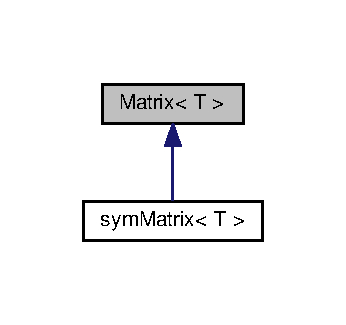
\includegraphics[width=166pt]{classMatrix__inherit__graph}
\end{center}
\end{figure}


Collaboration diagram for Matrix$<$ T $>$\+:\nopagebreak
\begin{figure}[H]
\begin{center}
\leavevmode
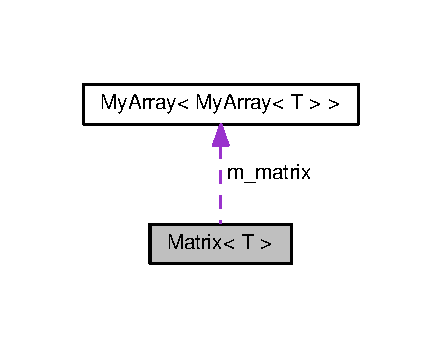
\includegraphics[width=212pt]{classMatrix__coll__graph}
\end{center}
\end{figure}
\subsection*{Public Member Functions}
\begin{DoxyCompactItemize}
\item 
\hyperlink{classMatrix_a9d567e3a121b1be0c3f9c461cab524fe}{Matrix} ()
\item 
\hyperlink{classMatrix_a19ffa179320a60ab6aeb0910f062895f}{Matrix} (const int n)
\item 
\hyperlink{classMatrix_a6a46705243036bfeee78fe2c84c54340}{Matrix} (const \hyperlink{classMatrix}{Matrix}$<$ T $>$ \&rhs)
\item 
\hyperlink{classMatrix_a91aa704de674203e96aece9e1955ccd3}{$\sim$\+Matrix} ()
\item 
virtual \hyperlink{classMatrix}{Matrix}$<$ T $>$ \& \hyperlink{classMatrix_a01990eb2552555d37c83272125be68e6}{operator=} (const \hyperlink{classMatrix}{Matrix}$<$ T $>$ \&rhs)
\item 
\hyperlink{classMatrix_ac503fc6ce19453907fd9ad85133fef39}{Matrix} (\hyperlink{classMatrix}{Matrix} \&\&rhs)
\item 
virtual \hyperlink{classMatrix}{Matrix}$<$ T $>$ \hyperlink{classMatrix_a9db4b4074daa2112eab910c7902fc5d9}{operator+} (const \hyperlink{classMatrix}{Matrix}$<$ T $>$ \&rhs) const 
\item 
virtual \hyperlink{classMatrix}{Matrix}$<$ T $>$ \hyperlink{classMatrix_a06a7f018ed353f0a8239a80ec8403be6}{operator-\/} (const \hyperlink{classMatrix}{Matrix}$<$ T $>$ \&rhs) const 
\item 
virtual \hyperlink{classMatrix}{Matrix}$<$ T $>$ \hyperlink{classMatrix_a358516deb804403fb91256a5a269d1e2}{operator$\ast$} (const \hyperlink{classMatrix}{Matrix}$<$ T $>$ \&rhs) const 
\item 
virtual \hyperlink{classMyArray}{My\+Array}$<$ T $>$ \hyperlink{classMatrix_a70c46247336f74291cc3e1b2fb800a34}{operator$\ast$} (const \hyperlink{classMyArray}{My\+Array}$<$ T $>$ \&rhs) const 
\item 
const \hyperlink{classMyArray}{My\+Array}$<$ T $>$ \& \hyperlink{classMatrix_a7b67f79f397146216c40197642ee4a44}{operator\mbox{[}$\,$\mbox{]}} (const int i) const 
\item 
\hyperlink{classMyArray}{My\+Array}$<$ T $>$ \& \hyperlink{classMatrix_a0d41726a8cfe08d0339f29a5b956f319}{operator\mbox{[}$\,$\mbox{]}} (const int i)
\item 
virtual void \hyperlink{classMatrix_aba8c673e5ca3bcc56a9bad1a1c0fed23}{scaler\+Multi} (const T scaler)
\item 
virtual void \hyperlink{classMatrix_a23bb949d4b4256dd253808e35d73d4b9}{switch\+Rows} (const int i, const int j)
\item 
\hyperlink{classMyArray}{My\+Array}$<$ \hyperlink{classMyArray}{My\+Array}$<$ T $>$ $>$ \hyperlink{classMatrix_afba2ee1c4e106b78099350d070ae1e51}{get\+Matrix} () const 
\item 
int \hyperlink{classMatrix_aa5d12d49bec4b4876f1a60c54a197ed7}{get\+Size} () const 
\item 
virtual void \hyperlink{classMatrix_a1add3e066eaaa19d5056fc6e2cbc767c}{set\+Size} (const int s)
\item 
virtual void \hyperlink{classMatrix_a0cf31a462707441cbbab037190c88f33}{set\+Matrix} (const int i, const int j, const T x)
\item 
\hyperlink{classMatrix}{Matrix}$<$ T $>$ \hyperlink{classMatrix_afe686234b6fe54ab2ae7f500777ca560}{transpose} () const 
\item 
virtual T \hyperlink{classMatrix_af786e95d49ae55d42c3bd6824a64e032}{operator()} (const int i, const int j) const 
\item 
virtual bool \hyperlink{classMatrix_ab5deedc9644d1b8c6bc220dd336f0102}{is\+Diag\+Dom} () const 
\end{DoxyCompactItemize}
\subsection*{Protected Member Functions}
\begin{DoxyCompactItemize}
\item 
void \hyperlink{classMatrix_ad39022f082bfee09e24d098796e14e10}{clear} ()
\end{DoxyCompactItemize}
\subsection*{Protected Attributes}
\begin{DoxyCompactItemize}
\item 
\hyperlink{classMyArray}{My\+Array}$<$ \hyperlink{classMyArray}{My\+Array}$<$ T $>$ $>$ \hyperlink{classMatrix_a3190abe45497430b3aa006002af3cb37}{m\+\_\+matrix}
\item 
int \hyperlink{classMatrix_a1113fd527e7677a93e88d1e736450968}{m\+\_\+size}
\end{DoxyCompactItemize}
\subsection*{Friends}
\begin{DoxyCompactItemize}
\item 
ostream \& \hyperlink{classMatrix_a7a26ce88f9d928002eba0af6847a0b44}{operator} (ostream \&out, \hyperlink{classMatrix}{Matrix}$<$ T $>$ \&mat)
\item 
istream \& \hyperlink{classMatrix_a175cb81129f42ab801259469bc7cc7a0}{operator$>$$>$} (istream \&in, \hyperlink{classMatrix}{Matrix}$<$ T $>$ \&mat)
\end{DoxyCompactItemize}


\subsection{Detailed Description}
\subsubsection*{template$<$class T$>$\\*
class Matrix$<$ T $>$}

\hyperlink{classMatrix}{Matrix} calss Reprents a NxN \hyperlink{classMatrix}{Matrix} contains a\+: m\+\_\+size -\/ represting the size of N m\+\_\+matrix -\/ an my\+Array of my\+Arrays represting the matrix 

\subsection{Constructor \& Destructor Documentation}
\index{Matrix@{Matrix}!Matrix@{Matrix}}
\index{Matrix@{Matrix}!Matrix@{Matrix}}
\subsubsection[{\texorpdfstring{Matrix()}{Matrix()}}]{\setlength{\rightskip}{0pt plus 5cm}template$<$typename T $>$ {\bf Matrix}$<$ T $>$\+::{\bf Matrix} (
\begin{DoxyParamCaption}
{}
\end{DoxyParamCaption}
)}\hypertarget{classMatrix_a9d567e3a121b1be0c3f9c461cab524fe}{}\label{classMatrix_a9d567e3a121b1be0c3f9c461cab524fe}
defult constructor. A new \hyperlink{classMatrix}{Matrix} is craeted with N equals 0. \begin{DoxyPrecond}{Precondition}
none 
\end{DoxyPrecond}
\begin{DoxyPostcond}{Postcondition}
a \hyperlink{classMatrix}{Matrix} is born! 
\end{DoxyPostcond}
\index{Matrix@{Matrix}!Matrix@{Matrix}}
\index{Matrix@{Matrix}!Matrix@{Matrix}}
\subsubsection[{\texorpdfstring{Matrix(const int n)}{Matrix(const int n)}}]{\setlength{\rightskip}{0pt plus 5cm}template$<$typename T $>$ {\bf Matrix}$<$ T $>$\+::{\bf Matrix} (
\begin{DoxyParamCaption}
\item[{const int}]{n}
\end{DoxyParamCaption}
)}\hypertarget{classMatrix_a19ffa179320a60ab6aeb0910f062895f}{}\label{classMatrix_a19ffa179320a60ab6aeb0910f062895f}
initialize constructor. A new \hyperlink{classMatrix}{Matrix} is craeted with dimensions equel to \char`\"{}n\char`\"{} \begin{DoxyPrecond}{Precondition}
size must be bigger then 0! Will throw a a length Error otherwise 
\end{DoxyPrecond}
\begin{DoxyPostcond}{Postcondition}
a \hyperlink{classMatrix}{Matrix} is born! 
\end{DoxyPostcond}
\index{Matrix@{Matrix}!Matrix@{Matrix}}
\index{Matrix@{Matrix}!Matrix@{Matrix}}
\subsubsection[{\texorpdfstring{Matrix(const Matrix$<$ T $>$ \&rhs)}{Matrix(const Matrix< T > &rhs)}}]{\setlength{\rightskip}{0pt plus 5cm}template$<$typename T $>$ {\bf Matrix}$<$ T $>$\+::{\bf Matrix} (
\begin{DoxyParamCaption}
\item[{const {\bf Matrix}$<$ T $>$ \&}]{rhs}
\end{DoxyParamCaption}
)}\hypertarget{classMatrix_a6a46705243036bfeee78fe2c84c54340}{}\label{classMatrix_a6a46705243036bfeee78fe2c84c54340}
copy constructor. A new Marix is craeted with size equel to R\+HS size. \begin{DoxyPrecond}{Precondition}
none 
\end{DoxyPrecond}
\begin{DoxyPostcond}{Postcondition}
a \hyperlink{classMatrix}{Matrix} is born! 
\end{DoxyPostcond}
\index{Matrix@{Matrix}!````~Matrix@{$\sim$\+Matrix}}
\index{````~Matrix@{$\sim$\+Matrix}!Matrix@{Matrix}}
\subsubsection[{\texorpdfstring{$\sim$\+Matrix()}{~Matrix()}}]{\setlength{\rightskip}{0pt plus 5cm}template$<$typename T $>$ {\bf Matrix}$<$ T $>$\+::$\sim${\bf Matrix} (
\begin{DoxyParamCaption}
{}
\end{DoxyParamCaption}
)}\hypertarget{classMatrix_a91aa704de674203e96aece9e1955ccd3}{}\label{classMatrix_a91aa704de674203e96aece9e1955ccd3}
deconstructor.

An Arnold Schwarzenegger Terminates the pointer to avoid Skynet taking over with their memorey Leacks. \char`\"{} Hasta La Vista , Pointer \char`\"{} \index{Matrix@{Matrix}!Matrix@{Matrix}}
\index{Matrix@{Matrix}!Matrix@{Matrix}}
\subsubsection[{\texorpdfstring{Matrix(\+Matrix \&\&rhs)}{Matrix(Matrix &&rhs)}}]{\setlength{\rightskip}{0pt plus 5cm}template$<$class T$>$ {\bf Matrix}$<$ T $>$\+::{\bf Matrix} (
\begin{DoxyParamCaption}
\item[{{\bf Matrix}$<$ T $>$ \&\&}]{rhs}
\end{DoxyParamCaption}
)\hspace{0.3cm}{\ttfamily [inline]}}\hypertarget{classMatrix_ac503fc6ce19453907fd9ad85133fef39}{}\label{classMatrix_ac503fc6ce19453907fd9ad85133fef39}
move constructor. A new \hyperlink{classMatrix}{Matrix} is craeted with Size equel to R\+HS size \begin{DoxyPrecond}{Precondition}
none 
\end{DoxyPrecond}
\begin{DoxyPostcond}{Postcondition}
a \hyperlink{classMatrix}{Matrix} is born! 
\end{DoxyPostcond}


\subsection{Member Function Documentation}
\index{Matrix@{Matrix}!clear@{clear}}
\index{clear@{clear}!Matrix@{Matrix}}
\subsubsection[{\texorpdfstring{clear()}{clear()}}]{\setlength{\rightskip}{0pt plus 5cm}template$<$typename T $>$ void {\bf Matrix}$<$ T $>$\+::clear (
\begin{DoxyParamCaption}
{}
\end{DoxyParamCaption}
)\hspace{0.3cm}{\ttfamily [protected]}}\hypertarget{classMatrix_ad39022f082bfee09e24d098796e14e10}{}\label{classMatrix_ad39022f082bfee09e24d098796e14e10}
clear dealoctes matrix \begin{DoxyPrecond}{Precondition}
none 
\end{DoxyPrecond}
\begin{DoxyPostcond}{Postcondition}
none 
\end{DoxyPostcond}
\index{Matrix@{Matrix}!get\+Matrix@{get\+Matrix}}
\index{get\+Matrix@{get\+Matrix}!Matrix@{Matrix}}
\subsubsection[{\texorpdfstring{get\+Matrix() const }{getMatrix() const }}]{\setlength{\rightskip}{0pt plus 5cm}template$<$class T$>$ {\bf My\+Array}$<${\bf My\+Array}$<$T$>$ $>$ {\bf Matrix}$<$ T $>$\+::get\+Matrix (
\begin{DoxyParamCaption}
{}
\end{DoxyParamCaption}
) const\hspace{0.3cm}{\ttfamily [inline]}}\hypertarget{classMatrix_afba2ee1c4e106b78099350d070ae1e51}{}\label{classMatrix_afba2ee1c4e106b78099350d070ae1e51}
get matrix returns m\+\_\+matrix \begin{DoxyPrecond}{Precondition}
none 
\end{DoxyPrecond}
\begin{DoxyPostcond}{Postcondition}
none 
\end{DoxyPostcond}
\index{Matrix@{Matrix}!get\+Size@{get\+Size}}
\index{get\+Size@{get\+Size}!Matrix@{Matrix}}
\subsubsection[{\texorpdfstring{get\+Size() const }{getSize() const }}]{\setlength{\rightskip}{0pt plus 5cm}template$<$class T$>$ int {\bf Matrix}$<$ T $>$\+::get\+Size (
\begin{DoxyParamCaption}
{}
\end{DoxyParamCaption}
) const\hspace{0.3cm}{\ttfamily [inline]}}\hypertarget{classMatrix_aa5d12d49bec4b4876f1a60c54a197ed7}{}\label{classMatrix_aa5d12d49bec4b4876f1a60c54a197ed7}
get size!

\begin{DoxyPrecond}{Precondition}
none 
\end{DoxyPrecond}
\begin{DoxyPostcond}{Postcondition}
none 
\end{DoxyPostcond}
\begin{DoxyReturn}{Returns}
size of Martix 
\end{DoxyReturn}
\index{Matrix@{Matrix}!is\+Diag\+Dom@{is\+Diag\+Dom}}
\index{is\+Diag\+Dom@{is\+Diag\+Dom}!Matrix@{Matrix}}
\subsubsection[{\texorpdfstring{is\+Diag\+Dom() const }{isDiagDom() const }}]{\setlength{\rightskip}{0pt plus 5cm}template$<$typename T $>$ bool {\bf Matrix}$<$ T $>$\+::is\+Diag\+Dom (
\begin{DoxyParamCaption}
{}
\end{DoxyParamCaption}
) const\hspace{0.3cm}{\ttfamily [virtual]}}\hypertarget{classMatrix_ab5deedc9644d1b8c6bc220dd336f0102}{}\label{classMatrix_ab5deedc9644d1b8c6bc220dd336f0102}
is diagonally dominant returns true if matrix is diagonally dominant. false otherwise. \begin{DoxyPrecond}{Precondition}
none 
\end{DoxyPrecond}
\begin{DoxyPostcond}{Postcondition}
none 
\end{DoxyPostcond}


Reimplemented in \hyperlink{classsymMatrix_a43d26e87d92d368544b9bd6384da8121}{sym\+Matrix$<$ T $>$}.

\index{Matrix@{Matrix}!operator()@{operator()}}
\index{operator()@{operator()}!Matrix@{Matrix}}
\subsubsection[{\texorpdfstring{operator()(const int i, const int j) const }{operator()(const int i, const int j) const }}]{\setlength{\rightskip}{0pt plus 5cm}template$<$typename T $>$ T {\bf Matrix}$<$ T $>$\+::{\bf operator}() (
\begin{DoxyParamCaption}
\item[{const int}]{i, }
\item[{const int}]{j}
\end{DoxyParamCaption}
) const\hspace{0.3cm}{\ttfamily [virtual]}}\hypertarget{classMatrix_af786e95d49ae55d42c3bd6824a64e032}{}\label{classMatrix_af786e95d49ae55d42c3bd6824a64e032}
operaotr () returns value of m\+\_\+matrix\mbox{[}i\mbox{]}\mbox{[}j\mbox{]} \begin{DoxyPrecond}{Precondition}
0 $<$ i,j $<$size 
\end{DoxyPrecond}
\begin{DoxyPostcond}{Postcondition}
none 
\end{DoxyPostcond}


Reimplemented in \hyperlink{classsymMatrix_a92bbf3194f8bf52559ee19ba706dd15c}{sym\+Matrix$<$ T $>$}.

\index{Matrix@{Matrix}!operator$\ast$@{operator$\ast$}}
\index{operator$\ast$@{operator$\ast$}!Matrix@{Matrix}}
\subsubsection[{\texorpdfstring{operator$\ast$(const Matrix$<$ T $>$ \&rhs) const }{operator*(const Matrix< T > &rhs) const }}]{\setlength{\rightskip}{0pt plus 5cm}template$<$typename T $>$ {\bf Matrix}$<$ T $>$ {\bf Matrix}$<$ T $>$\+::{\bf operator}$\ast$ (
\begin{DoxyParamCaption}
\item[{const {\bf Matrix}$<$ T $>$ \&}]{rhs}
\end{DoxyParamCaption}
) const\hspace{0.3cm}{\ttfamily [virtual]}}\hypertarget{classMatrix_a358516deb804403fb91256a5a269d1e2}{}\label{classMatrix_a358516deb804403fb91256a5a269d1e2}
\hyperlink{classMatrix}{Matrix} multiplication caclualtes the multiplication of 2 matrixs and returens a new matrix with the calculated values \begin{DoxyPrecond}{Precondition}
size of CO must be equel to rhs, Will throw a a length Error otherwise. \char`\"{}$\ast$\char`\"{} binary operator must be defiend for T. 
\end{DoxyPrecond}
\begin{DoxyPostcond}{Postcondition}
a matrix is born! 
\end{DoxyPostcond}


Reimplemented in \hyperlink{classsymMatrix_a4c1a9a20ab9bd68aca9f9d35d25e0e36}{sym\+Matrix$<$ T $>$}.

\index{Matrix@{Matrix}!operator$\ast$@{operator$\ast$}}
\index{operator$\ast$@{operator$\ast$}!Matrix@{Matrix}}
\subsubsection[{\texorpdfstring{operator$\ast$(const My\+Array$<$ T $>$ \&rhs) const }{operator*(const MyArray< T > &rhs) const }}]{\setlength{\rightskip}{0pt plus 5cm}template$<$typename T $>$ {\bf My\+Array}$<$ T $>$ {\bf Matrix}$<$ T $>$\+::{\bf operator}$\ast$ (
\begin{DoxyParamCaption}
\item[{const {\bf My\+Array}$<$ T $>$ \&}]{rhs}
\end{DoxyParamCaption}
) const\hspace{0.3cm}{\ttfamily [virtual]}}\hypertarget{classMatrix_a70c46247336f74291cc3e1b2fb800a34}{}\label{classMatrix_a70c46247336f74291cc3e1b2fb800a34}
\hyperlink{classMatrix}{Matrix} -\/ Vector multiplication caclualtes the multiplication of 2 of a \hyperlink{classMatrix}{Matrix} with an Array and returens a new Vector with the calculated values \begin{DoxyPrecond}{Precondition}
size of CO must be equel to rhs array size! Will throw a a length Error otherwise. \char`\"{}$\ast$\char`\"{} binary operator must be defiend for T. 
\end{DoxyPrecond}
\begin{DoxyPostcond}{Postcondition}
a Vector is born! 
\end{DoxyPostcond}


Reimplemented in \hyperlink{classsymMatrix_aa7adbc9378944126e08af6072ff648eb}{sym\+Matrix$<$ T $>$}.

\index{Matrix@{Matrix}!operator+@{operator+}}
\index{operator+@{operator+}!Matrix@{Matrix}}
\subsubsection[{\texorpdfstring{operator+(const Matrix$<$ T $>$ \&rhs) const }{operator+(const Matrix< T > &rhs) const }}]{\setlength{\rightskip}{0pt plus 5cm}template$<$typename T $>$ {\bf Matrix}$<$ T $>$ {\bf Matrix}$<$ T $>$\+::{\bf operator}+ (
\begin{DoxyParamCaption}
\item[{const {\bf Matrix}$<$ T $>$ \&}]{rhs}
\end{DoxyParamCaption}
) const\hspace{0.3cm}{\ttfamily [virtual]}}\hypertarget{classMatrix_a9db4b4074daa2112eab910c7902fc5d9}{}\label{classMatrix_a9db4b4074daa2112eab910c7902fc5d9}

\begin{DoxyItemize}
\item operator adds the sum of CO to rhs, retures a new \hyperlink{classMatrix}{Matrix} with the calculated values \begin{DoxyPrecond}{Precondition}
size of CO must be equel to rhs, Will throw a a length Error otherwise. \char`\"{}+\char`\"{} binary operator must be defiend for T. 
\end{DoxyPrecond}
\begin{DoxyPostcond}{Postcondition}
a matrix is born! 
\end{DoxyPostcond}

\end{DoxyItemize}

Reimplemented in \hyperlink{classsymMatrix_a47071a21daf752e9a378c593ef85dbb2}{sym\+Matrix$<$ T $>$}.

\index{Matrix@{Matrix}!operator-\/@{operator-\/}}
\index{operator-\/@{operator-\/}!Matrix@{Matrix}}
\subsubsection[{\texorpdfstring{operator-\/(const Matrix$<$ T $>$ \&rhs) const }{operator-(const Matrix< T > &rhs) const }}]{\setlength{\rightskip}{0pt plus 5cm}template$<$typename T $>$ {\bf Matrix}$<$ T $>$ {\bf Matrix}$<$ T $>$\+::{\bf operator}-\/ (
\begin{DoxyParamCaption}
\item[{const {\bf Matrix}$<$ T $>$ \&}]{rhs}
\end{DoxyParamCaption}
) const\hspace{0.3cm}{\ttfamily [virtual]}}\hypertarget{classMatrix_a06a7f018ed353f0a8239a80ec8403be6}{}\label{classMatrix_a06a7f018ed353f0a8239a80ec8403be6}

\begin{DoxyItemize}
\item operator caclualtes the differnce of CO to rhs, retures a new \hyperlink{classMatrix}{Matrix} with the calculated values \begin{DoxyPrecond}{Precondition}
size of CO must be equel to rhs, Will throw a a length Error otherwise. \char`\"{}-\/\char`\"{} binary operator must be defiend for T. 
\end{DoxyPrecond}
\begin{DoxyPostcond}{Postcondition}
a matrix is born! 
\end{DoxyPostcond}

\end{DoxyItemize}

Reimplemented in \hyperlink{classsymMatrix_aaa418f9273ccc5da9d01c645e78ef657}{sym\+Matrix$<$ T $>$}.

\index{Matrix@{Matrix}!operator=@{operator=}}
\index{operator=@{operator=}!Matrix@{Matrix}}
\subsubsection[{\texorpdfstring{operator=(const Matrix$<$ T $>$ \&rhs)}{operator=(const Matrix< T > &rhs)}}]{\setlength{\rightskip}{0pt plus 5cm}template$<$typename T $>$ {\bf Matrix}$<$ T $>$ \& {\bf Matrix}$<$ T $>$\+::{\bf operator}= (
\begin{DoxyParamCaption}
\item[{const {\bf Matrix}$<$ T $>$ \&}]{rhs}
\end{DoxyParamCaption}
)\hspace{0.3cm}{\ttfamily [virtual]}}\hypertarget{classMatrix_a01990eb2552555d37c83272125be68e6}{}\label{classMatrix_a01990eb2552555d37c83272125be68e6}
= assignment turns the CO \hyperlink{classMatrix}{Matrix} into R\+HS matix \begin{DoxyPrecond}{Precondition}
none 
\end{DoxyPrecond}
\begin{DoxyPostcond}{Postcondition}
none 
\end{DoxyPostcond}
\index{Matrix@{Matrix}!operator\mbox{[}$\,$\mbox{]}@{operator[]}}
\index{operator\mbox{[}$\,$\mbox{]}@{operator[]}!Matrix@{Matrix}}
\subsubsection[{\texorpdfstring{operator[](const int i) const }{operator[](const int i) const }}]{\setlength{\rightskip}{0pt plus 5cm}template$<$typename T $>$ const {\bf My\+Array}$<$ T $>$ \& {\bf Matrix}$<$ T $>$\+::{\bf operator}\mbox{[}$\,$\mbox{]} (
\begin{DoxyParamCaption}
\item[{const int}]{i}
\end{DoxyParamCaption}
) const}\hypertarget{classMatrix_a7b67f79f397146216c40197642ee4a44}{}\label{classMatrix_a7b67f79f397146216c40197642ee4a44}
object getter \mbox{[}\mbox{]} const

\begin{DoxyPrecond}{Precondition}
0 $<$ i $<$ size, will throw a a length Error otherwise 
\end{DoxyPrecond}
\begin{DoxyPostcond}{Postcondition}
none 
\end{DoxyPostcond}
\begin{DoxyReturn}{Returns}
Will return the \hyperlink{classMyArray}{My\+Array} at index i. 
\end{DoxyReturn}
\index{Matrix@{Matrix}!operator\mbox{[}$\,$\mbox{]}@{operator[]}}
\index{operator\mbox{[}$\,$\mbox{]}@{operator[]}!Matrix@{Matrix}}
\subsubsection[{\texorpdfstring{operator[](const int i)}{operator[](const int i)}}]{\setlength{\rightskip}{0pt plus 5cm}template$<$typename T $>$ {\bf My\+Array}$<$ T $>$ \& {\bf Matrix}$<$ T $>$\+::{\bf operator}\mbox{[}$\,$\mbox{]} (
\begin{DoxyParamCaption}
\item[{const int}]{i}
\end{DoxyParamCaption}
)}\hypertarget{classMatrix_a0d41726a8cfe08d0339f29a5b956f319}{}\label{classMatrix_a0d41726a8cfe08d0339f29a5b956f319}
object getter \mbox{[}\mbox{]} non-\/const

\begin{DoxyPrecond}{Precondition}
0 $<$ i $<$ size, will throw a a length Error otherwise 
\end{DoxyPrecond}
\begin{DoxyPostcond}{Postcondition}
none 
\end{DoxyPostcond}
\begin{DoxyReturn}{Returns}
Will return the \hyperlink{classMyArray}{My\+Array} at index i. 
\end{DoxyReturn}
\index{Matrix@{Matrix}!scaler\+Multi@{scaler\+Multi}}
\index{scaler\+Multi@{scaler\+Multi}!Matrix@{Matrix}}
\subsubsection[{\texorpdfstring{scaler\+Multi(const T scaler)}{scalerMulti(const T scaler)}}]{\setlength{\rightskip}{0pt plus 5cm}template$<$typename T $>$ void {\bf Matrix}$<$ T $>$\+::scaler\+Multi (
\begin{DoxyParamCaption}
\item[{const T}]{scaler}
\end{DoxyParamCaption}
)\hspace{0.3cm}{\ttfamily [virtual]}}\hypertarget{classMatrix_aba8c673e5ca3bcc56a9bad1a1c0fed23}{}\label{classMatrix_aba8c673e5ca3bcc56a9bad1a1c0fed23}
\hyperlink{classMatrix}{Matrix} Scaler multiplication caclualtes the multiplication of a matrixs with a scaler and modifies the CO m\+\_\+matrix with calculation \begin{DoxyPrecond}{Precondition}
\char`\"{}$\ast$\char`\"{} binary operator must be defiend for T. 
\end{DoxyPrecond}
\begin{DoxyPostcond}{Postcondition}
none 
\end{DoxyPostcond}


Reimplemented in \hyperlink{classsymMatrix_a75cb07e28a2ef936e45a7e3324429667}{sym\+Matrix$<$ T $>$}.

\index{Matrix@{Matrix}!set\+Matrix@{set\+Matrix}}
\index{set\+Matrix@{set\+Matrix}!Matrix@{Matrix}}
\subsubsection[{\texorpdfstring{set\+Matrix(const int i, const int j, const T x)}{setMatrix(const int i, const int j, const T x)}}]{\setlength{\rightskip}{0pt plus 5cm}template$<$typename T $>$ void {\bf Matrix}$<$ T $>$\+::set\+Matrix (
\begin{DoxyParamCaption}
\item[{const int}]{i, }
\item[{const int}]{j, }
\item[{const T}]{x}
\end{DoxyParamCaption}
)\hspace{0.3cm}{\ttfamily [virtual]}}\hypertarget{classMatrix_a0cf31a462707441cbbab037190c88f33}{}\label{classMatrix_a0cf31a462707441cbbab037190c88f33}
set matrix! changes value of m\+\_\+matrix\mbox{[}i\mbox{]}\mbox{[}j\mbox{]} to x \begin{DoxyPrecond}{Precondition}
0 $<$ i,j $<$ size. 
\end{DoxyPrecond}
\begin{DoxyPostcond}{Postcondition}
m\+\_\+matrix modified 
\end{DoxyPostcond}


Reimplemented in \hyperlink{classsymMatrix_a28d1f286c0a8572a26441afd635cba51}{sym\+Matrix$<$ T $>$}.

\index{Matrix@{Matrix}!set\+Size@{set\+Size}}
\index{set\+Size@{set\+Size}!Matrix@{Matrix}}
\subsubsection[{\texorpdfstring{set\+Size(const int s)}{setSize(const int s)}}]{\setlength{\rightskip}{0pt plus 5cm}template$<$typename T $>$ void {\bf Matrix}$<$ T $>$\+::set\+Size (
\begin{DoxyParamCaption}
\item[{const int}]{s}
\end{DoxyParamCaption}
)\hspace{0.3cm}{\ttfamily [virtual]}}\hypertarget{classMatrix_a1add3e066eaaa19d5056fc6e2cbc767c}{}\label{classMatrix_a1add3e066eaaa19d5056fc6e2cbc767c}
set size!

\begin{DoxyPrecond}{Precondition}
s must be postive 
\end{DoxyPrecond}
\begin{DoxyPostcond}{Postcondition}
none 
\end{DoxyPostcond}


Reimplemented in \hyperlink{classsymMatrix_a06379c2668a6b1fba8b133d753a8f57c}{sym\+Matrix$<$ T $>$}.

\index{Matrix@{Matrix}!switch\+Rows@{switch\+Rows}}
\index{switch\+Rows@{switch\+Rows}!Matrix@{Matrix}}
\subsubsection[{\texorpdfstring{switch\+Rows(const int i, const int j)}{switchRows(const int i, const int j)}}]{\setlength{\rightskip}{0pt plus 5cm}template$<$typename T $>$ void {\bf Matrix}$<$ T $>$\+::switch\+Rows (
\begin{DoxyParamCaption}
\item[{const int}]{i, }
\item[{const int}]{j}
\end{DoxyParamCaption}
)\hspace{0.3cm}{\ttfamily [virtual]}}\hypertarget{classMatrix_a23bb949d4b4256dd253808e35d73d4b9}{}\label{classMatrix_a23bb949d4b4256dd253808e35d73d4b9}
Row switcher switches the array at index i with array at index j and vice versa \begin{DoxyPrecond}{Precondition}
0 $<$ i,j $<$ m\+\_\+size, will throw a a length Error otherwise 
\end{DoxyPrecond}
\begin{DoxyPostcond}{Postcondition}
none 
\end{DoxyPostcond}
\index{Matrix@{Matrix}!transpose@{transpose}}
\index{transpose@{transpose}!Matrix@{Matrix}}
\subsubsection[{\texorpdfstring{transpose() const }{transpose() const }}]{\setlength{\rightskip}{0pt plus 5cm}template$<$typename T $>$ {\bf Matrix}$<$ T $>$ {\bf Matrix}$<$ T $>$\+::transpose (
\begin{DoxyParamCaption}
{}
\end{DoxyParamCaption}
) const}\hypertarget{classMatrix_afe686234b6fe54ab2ae7f500777ca560}{}\label{classMatrix_afe686234b6fe54ab2ae7f500777ca560}
\hyperlink{classMatrix}{Matrix} transpose calculator Creates a new matrix with is a trasposed version of the CO \begin{DoxyPrecond}{Precondition}
none 
\end{DoxyPrecond}
\begin{DoxyPostcond}{Postcondition}
a \hyperlink{classMatrix}{Matrix} is born 
\end{DoxyPostcond}


\subsection{Friends And Related Function Documentation}
\index{Matrix@{Matrix}!operator@{operator}}
\index{operator@{operator}!Matrix@{Matrix}}
\subsubsection[{\texorpdfstring{operator}{operator}}]{\setlength{\rightskip}{0pt plus 5cm}template$<$class T$>$ ostream\& operator (
\begin{DoxyParamCaption}
\item[{ostream \&}]{out, }
\item[{{\bf Matrix}$<$ T $>$ \&}]{mat}
\end{DoxyParamCaption}
)\hspace{0.3cm}{\ttfamily [friend]}}\hypertarget{classMatrix_a7a26ce88f9d928002eba0af6847a0b44}{}\label{classMatrix_a7a26ce88f9d928002eba0af6847a0b44}
Stream insertion operator for {\ttfamily \hyperlink{classMatrix}{Matrix}}.

\begin{DoxyPrecond}{Precondition}
Stream insertion operator is defined for {\ttfamily T}. 
\end{DoxyPrecond}
\begin{DoxyPostcond}{Postcondition}
The contents of the m\+\_\+matrix are printed to the ouptut stream. Each array is printed on a new row. 
\end{DoxyPostcond}
\begin{DoxyReturn}{Returns}
the modified output stream. 
\end{DoxyReturn}
\index{Matrix@{Matrix}!operator$>$$>$@{operator$>$$>$}}
\index{operator$>$$>$@{operator$>$$>$}!Matrix@{Matrix}}
\subsubsection[{\texorpdfstring{operator$>$$>$}{operator>>}}]{\setlength{\rightskip}{0pt plus 5cm}template$<$class T$>$ istream\& {\bf operator}$>$$>$ (
\begin{DoxyParamCaption}
\item[{istream \&}]{in, }
\item[{{\bf Matrix}$<$ T $>$ \&}]{mat}
\end{DoxyParamCaption}
)\hspace{0.3cm}{\ttfamily [friend]}}\hypertarget{classMatrix_a175cb81129f42ab801259469bc7cc7a0}{}\label{classMatrix_a175cb81129f42ab801259469bc7cc7a0}
Stream insertion operator for {\ttfamily \hyperlink{classMatrix}{Matrix}}.

\begin{DoxyPrecond}{Precondition}
Stream insertion operator is defined for {\ttfamily T}. 
\end{DoxyPrecond}
\begin{DoxyPostcond}{Postcondition}
the m\+\_\+matrix if filled with the input 
\end{DoxyPostcond}
\begin{DoxyReturn}{Returns}
the modified input stream. 
\end{DoxyReturn}


\subsection{Member Data Documentation}
\index{Matrix@{Matrix}!m\+\_\+matrix@{m\+\_\+matrix}}
\index{m\+\_\+matrix@{m\+\_\+matrix}!Matrix@{Matrix}}
\subsubsection[{\texorpdfstring{m\+\_\+matrix}{m_matrix}}]{\setlength{\rightskip}{0pt plus 5cm}template$<$class T$>$ {\bf My\+Array}$<${\bf My\+Array}$<$T$>$ $>$ {\bf Matrix}$<$ T $>$\+::m\+\_\+matrix\hspace{0.3cm}{\ttfamily [protected]}}\hypertarget{classMatrix_a3190abe45497430b3aa006002af3cb37}{}\label{classMatrix_a3190abe45497430b3aa006002af3cb37}
the matrix (Array of array\textquotesingle{}s) \index{Matrix@{Matrix}!m\+\_\+size@{m\+\_\+size}}
\index{m\+\_\+size@{m\+\_\+size}!Matrix@{Matrix}}
\subsubsection[{\texorpdfstring{m\+\_\+size}{m_size}}]{\setlength{\rightskip}{0pt plus 5cm}template$<$class T$>$ int {\bf Matrix}$<$ T $>$\+::m\+\_\+size\hspace{0.3cm}{\ttfamily [protected]}}\hypertarget{classMatrix_a1113fd527e7677a93e88d1e736450968}{}\label{classMatrix_a1113fd527e7677a93e88d1e736450968}
size var 

The documentation for this class was generated from the following files\+:\begin{DoxyCompactItemize}
\item 
\hyperlink{matrix_8h}{matrix.\+h}\item 
matrix.\+hpp\end{DoxyCompactItemize}

\hypertarget{classmesh}{}\section{mesh$<$ T $>$ Class Template Reference}
\label{classmesh}\index{mesh$<$ T $>$@{mesh$<$ T $>$}}


{\ttfamily \#include $<$mesh.\+h$>$}

\subsection*{Public Member Functions}
\begin{DoxyCompactItemize}
\item 
\hyperlink{classmesh_a869958b6eceb09e8313bce70c3e8dc53}{mesh} (const int size)
\item 
\hyperlink{classsymMatrix}{sym\+Matrix}$<$ T $>$ \& \hyperlink{classmesh_a667fed9c4c02fe4acd2b4043aadc216d}{get\+Mesh\+\_\+mat} ()
\item 
\hyperlink{classMyArray}{My\+Array}$<$ T $>$ \& \hyperlink{classmesh_adee2e789ef5178b84d3bed2a27a4eb7f}{get\+Mesh\+\_\+vect} ()
\end{DoxyCompactItemize}


\subsection{Detailed Description}
\subsubsection*{template$<$typename T$>$\\*
class mesh$<$ T $>$}

the Mesh calculation class 

\subsection{Constructor \& Destructor Documentation}
\index{mesh@{mesh}!mesh@{mesh}}
\index{mesh@{mesh}!mesh@{mesh}}
\subsubsection[{\texorpdfstring{mesh(const int size)}{mesh(const int size)}}]{\setlength{\rightskip}{0pt plus 5cm}template$<$typename T $>$ {\bf mesh}$<$ T $>$\+::{\bf mesh} (
\begin{DoxyParamCaption}
\item[{const int}]{size}
\end{DoxyParamCaption}
)}\hypertarget{classmesh_a869958b6eceb09e8313bce70c3e8dc53}{}\label{classmesh_a869958b6eceb09e8313bce70c3e8dc53}
initilze constructor functinos creates Poisson’s Vector and \hyperlink{classMatrix}{Matrix} with given size \begin{DoxyPrecond}{Precondition}
size must be greater then 0. Throws length error otherwise "mesh\+\_\+vect\char`\"{} is modfied. \char`\"{}mesh\+\_\+mat" is modfied. 
\end{DoxyPrecond}


\subsection{Member Function Documentation}
\index{mesh@{mesh}!get\+Mesh\+\_\+mat@{get\+Mesh\+\_\+mat}}
\index{get\+Mesh\+\_\+mat@{get\+Mesh\+\_\+mat}!mesh@{mesh}}
\subsubsection[{\texorpdfstring{get\+Mesh\+\_\+mat()}{getMesh_mat()}}]{\setlength{\rightskip}{0pt plus 5cm}template$<$typename T $>$ {\bf sym\+Matrix}$<$T$>$\& {\bf mesh}$<$ T $>$\+::get\+Mesh\+\_\+mat (
\begin{DoxyParamCaption}
{}
\end{DoxyParamCaption}
)\hspace{0.3cm}{\ttfamily [inline]}}\hypertarget{classmesh_a667fed9c4c02fe4acd2b4043aadc216d}{}\label{classmesh_a667fed9c4c02fe4acd2b4043aadc216d}
get\+Mesh\+\_\+mat retuerns mesh\+\_\+mat \begin{DoxyPrecond}{Precondition}
none 
\end{DoxyPrecond}
\begin{DoxyPostcond}{Postcondition}
none 
\end{DoxyPostcond}
\index{mesh@{mesh}!get\+Mesh\+\_\+vect@{get\+Mesh\+\_\+vect}}
\index{get\+Mesh\+\_\+vect@{get\+Mesh\+\_\+vect}!mesh@{mesh}}
\subsubsection[{\texorpdfstring{get\+Mesh\+\_\+vect()}{getMesh_vect()}}]{\setlength{\rightskip}{0pt plus 5cm}template$<$typename T $>$ {\bf My\+Array}$<$T$>$\& {\bf mesh}$<$ T $>$\+::get\+Mesh\+\_\+vect (
\begin{DoxyParamCaption}
{}
\end{DoxyParamCaption}
)\hspace{0.3cm}{\ttfamily [inline]}}\hypertarget{classmesh_adee2e789ef5178b84d3bed2a27a4eb7f}{}\label{classmesh_adee2e789ef5178b84d3bed2a27a4eb7f}
get\+Mesh\+\_\+vect retuerns mesh\+\_\+vect \begin{DoxyPrecond}{Precondition}
none 
\end{DoxyPrecond}
\begin{DoxyPostcond}{Postcondition}
none 
\end{DoxyPostcond}


The documentation for this class was generated from the following files\+:\begin{DoxyCompactItemize}
\item 
\hyperlink{mesh_8h}{mesh.\+h}\item 
mesh.\+hpp\end{DoxyCompactItemize}

\hypertarget{classMyArray}{}\section{My\+Array$<$ T $>$ Class Template Reference}
\label{classMyArray}\index{My\+Array$<$ T $>$@{My\+Array$<$ T $>$}}


{\ttfamily \#include $<$my\+Array.\+h$>$}

\subsection*{Public Member Functions}
\begin{DoxyCompactItemize}
\item 
\hyperlink{classMyArray_a5e2f56ae6e3b87c1635bedf8b4b76fb9}{My\+Array} (const int size)
\item 
\hyperlink{classMyArray_acb3cd41349cf47f00e119061894929a6}{My\+Array} ()
\item 
\hyperlink{classMyArray_a03c11ccacb545bdcaf686747d3dc741d}{My\+Array} (const \hyperlink{classMyArray}{My\+Array}$<$ T $>$ \&rhs)
\item 
\hyperlink{classMyArray_a614502f17fa14578ed29c99cb9a9861e}{My\+Array} (\hyperlink{classMyArray}{My\+Array} \&\&rhs)
\item 
\hyperlink{classMyArray_a55bc32d921ca509c9820549cb8baac22}{$\sim$\+My\+Array} ()
\item 
T \& \hyperlink{classMyArray_a29386688c63b9c7694fcaea57e772781}{operator\mbox{[}$\,$\mbox{]}} (const int index) const 
\item 
int \hyperlink{classMyArray_a0b7673af1b2f8d69f9345b3fd817cce4}{get\+Size} () const 
\item 
void \hyperlink{classMyArray_ab2e0c78689ddcfd142dbef361b7c0339}{set\+Size} (const int n)
\item 
void \hyperlink{classMyArray_a631fd2535793febd2f7acd7c70ca94b6}{clear} ()
\item 
\hyperlink{classMyArray}{My\+Array}$<$ T $>$ \& \hyperlink{classMyArray_a2f16f482ff8b1f600d288a9ca04c2658}{operator=} (const \hyperlink{classMyArray}{My\+Array}$<$ T $>$ \&rhs)
\item 
\hyperlink{classMyArray}{My\+Array}$<$ T $>$ \& \hyperlink{classMyArray_a04128aefb2c6a87d84cc29fdc6aeade7}{operator=} (const T)
\item 
void \hyperlink{classMyArray_a0c00635e4361df03eff1c371c1ab5567}{insert} (const T \&x, int pos)
\item 
bool \hyperlink{classMyArray_a75f3601d5480f089016a20eb3a1d3918}{is\+Zero\+Vec} ()
\item 
T \hyperlink{classMyArray_a491463a1b65467564e572c005bdc38df}{operator$\ast$} (const \hyperlink{classMyArray}{My\+Array}$<$ T $>$ \&rhs) const 
\item 
\hyperlink{classMyArray}{My\+Array}$<$ T $>$ \hyperlink{classMyArray_a65f0252bd35555144a102fe5c4e30629}{operator$\ast$} (const T \&scaler) const 
\item 
\hyperlink{classMyArray}{My\+Array}$<$ T $>$ \hyperlink{classMyArray_ae409f4dbb669a3993c7ea2099ca9076a}{operator+} (const \hyperlink{classMyArray}{My\+Array}$<$ T $>$ \&rhs) const 
\item 
\hyperlink{classMyArray}{My\+Array}$<$ T $>$ \hyperlink{classMyArray_a681601413d5b03d3319959186537430c}{operator-\/} (const \hyperlink{classMyArray}{My\+Array}$<$ T $>$ \&rhs) const 
\end{DoxyCompactItemize}
\subsection*{Friends}
\begin{DoxyCompactItemize}
\item 
ostream \& \hyperlink{classMyArray_a8568f8eed1d6c6b506aed173e9cb9326}{operator} (ostream \&out, const \hyperlink{classMyArray}{My\+Array}$<$ T $>$ \&arr)
\end{DoxyCompactItemize}


\subsection{Detailed Description}
\subsubsection*{template$<$class T$>$\\*
class My\+Array$<$ T $>$}

my\+Array calss

contains a\+: m\+\_\+size -\/ represting the size of the array ptr\+\_\+to\+\_\+data -\/ a pointer to the beginning of the array 

\subsection{Constructor \& Destructor Documentation}
\index{My\+Array@{My\+Array}!My\+Array@{My\+Array}}
\index{My\+Array@{My\+Array}!My\+Array@{My\+Array}}
\subsubsection[{\texorpdfstring{My\+Array(const int size)}{MyArray(const int size)}}]{\setlength{\rightskip}{0pt plus 5cm}template$<$typename T $>$ {\bf My\+Array}$<$ T $>$\+::{\bf My\+Array} (
\begin{DoxyParamCaption}
\item[{const int}]{size}
\end{DoxyParamCaption}
)}\hypertarget{classMyArray_a5e2f56ae6e3b87c1635bedf8b4b76fb9}{}\label{classMyArray_a5e2f56ae6e3b87c1635bedf8b4b76fb9}
initialize constructor. A new Array is craeted length equel \char`\"{}size\char`\"{} \begin{DoxyPrecond}{Precondition}
size must be bigger then 0! Will throw a a length Error otherwise 
\end{DoxyPrecond}
\begin{DoxyPostcond}{Postcondition}
a \hyperlink{classMyArray}{My\+Array} is born! 
\end{DoxyPostcond}
\index{My\+Array@{My\+Array}!My\+Array@{My\+Array}}
\index{My\+Array@{My\+Array}!My\+Array@{My\+Array}}
\subsubsection[{\texorpdfstring{My\+Array()}{MyArray()}}]{\setlength{\rightskip}{0pt plus 5cm}template$<$typename T $>$ {\bf My\+Array}$<$ T $>$\+::{\bf My\+Array} (
\begin{DoxyParamCaption}
{}
\end{DoxyParamCaption}
)}\hypertarget{classMyArray_acb3cd41349cf47f00e119061894929a6}{}\label{classMyArray_acb3cd41349cf47f00e119061894929a6}
defult constructor. A new Array is craeted with size 0 and ptr\+\_\+to\+\_\+data points to 0. \begin{DoxyPrecond}{Precondition}
none 
\end{DoxyPrecond}
\begin{DoxyPostcond}{Postcondition}
a \hyperlink{classMyArray}{My\+Array} is born! 
\end{DoxyPostcond}
\index{My\+Array@{My\+Array}!My\+Array@{My\+Array}}
\index{My\+Array@{My\+Array}!My\+Array@{My\+Array}}
\subsubsection[{\texorpdfstring{My\+Array(const My\+Array$<$ T $>$ \&rhs)}{MyArray(const MyArray< T > &rhs)}}]{\setlength{\rightskip}{0pt plus 5cm}template$<$typename T$>$ {\bf My\+Array}$<$ T $>$\+::{\bf My\+Array} (
\begin{DoxyParamCaption}
\item[{const {\bf My\+Array}$<$ T $>$ \&}]{rhs}
\end{DoxyParamCaption}
)}\hypertarget{classMyArray_a03c11ccacb545bdcaf686747d3dc741d}{}\label{classMyArray_a03c11ccacb545bdcaf686747d3dc741d}
copy constructor. A new Array is craeted length equel to R\+HS size. New array does N\+OT point to same adress as R\+HS. \begin{DoxyPrecond}{Precondition}

\end{DoxyPrecond}
\begin{DoxyPostcond}{Postcondition}
a \hyperlink{classMyArray}{My\+Array} is born! 
\end{DoxyPostcond}
\index{My\+Array@{My\+Array}!My\+Array@{My\+Array}}
\index{My\+Array@{My\+Array}!My\+Array@{My\+Array}}
\subsubsection[{\texorpdfstring{My\+Array(\+My\+Array \&\&rhs)}{MyArray(MyArray &&rhs)}}]{\setlength{\rightskip}{0pt plus 5cm}template$<$class T$>$ {\bf My\+Array}$<$ T $>$\+::{\bf My\+Array} (
\begin{DoxyParamCaption}
\item[{{\bf My\+Array}$<$ T $>$ \&\&}]{rhs}
\end{DoxyParamCaption}
)\hspace{0.3cm}{\ttfamily [inline]}}\hypertarget{classMyArray_a614502f17fa14578ed29c99cb9a9861e}{}\label{classMyArray_a614502f17fa14578ed29c99cb9a9861e}
move constructor. A new Array is craeted length equel to R\+HS size. New array does N\+OT point to same adress as R\+HS. \begin{DoxyPrecond}{Precondition}

\end{DoxyPrecond}
\begin{DoxyPostcond}{Postcondition}
a \hyperlink{classMyArray}{My\+Array} is born! 
\end{DoxyPostcond}
\index{My\+Array@{My\+Array}!````~My\+Array@{$\sim$\+My\+Array}}
\index{````~My\+Array@{$\sim$\+My\+Array}!My\+Array@{My\+Array}}
\subsubsection[{\texorpdfstring{$\sim$\+My\+Array()}{~MyArray()}}]{\setlength{\rightskip}{0pt plus 5cm}template$<$typename T $>$ {\bf My\+Array}$<$ T $>$\+::$\sim${\bf My\+Array} (
\begin{DoxyParamCaption}
{}
\end{DoxyParamCaption}
)}\hypertarget{classMyArray_a55bc32d921ca509c9820549cb8baac22}{}\label{classMyArray_a55bc32d921ca509c9820549cb8baac22}
deconstructor.

An Arnold Schwarzenegger Terminates the pointer to avoid Skynet taking over with their memorey Leacks. \char`\"{} Hasta La Vista , Pointer \char`\"{} 

\subsection{Member Function Documentation}
\index{My\+Array@{My\+Array}!clear@{clear}}
\index{clear@{clear}!My\+Array@{My\+Array}}
\subsubsection[{\texorpdfstring{clear()}{clear()}}]{\setlength{\rightskip}{0pt plus 5cm}template$<$typename T $>$ void {\bf My\+Array}$<$ T $>$\+::clear (
\begin{DoxyParamCaption}
{}
\end{DoxyParamCaption}
)}\hypertarget{classMyArray_a631fd2535793febd2f7acd7c70ca94b6}{}\label{classMyArray_a631fd2535793febd2f7acd7c70ca94b6}
clear emptys out the array! \begin{DoxyPrecond}{Precondition}
none 
\end{DoxyPrecond}
\begin{DoxyPostcond}{Postcondition}
ptr\+\_\+to\+\_\+data points to 0 
\end{DoxyPostcond}
\index{My\+Array@{My\+Array}!get\+Size@{get\+Size}}
\index{get\+Size@{get\+Size}!My\+Array@{My\+Array}}
\subsubsection[{\texorpdfstring{get\+Size() const }{getSize() const }}]{\setlength{\rightskip}{0pt plus 5cm}template$<$class T$>$ int {\bf My\+Array}$<$ T $>$\+::get\+Size (
\begin{DoxyParamCaption}
{}
\end{DoxyParamCaption}
) const\hspace{0.3cm}{\ttfamily [inline]}}\hypertarget{classMyArray_a0b7673af1b2f8d69f9345b3fd817cce4}{}\label{classMyArray_a0b7673af1b2f8d69f9345b3fd817cce4}
get size!

\begin{DoxyPrecond}{Precondition}
none 
\end{DoxyPrecond}
\begin{DoxyPostcond}{Postcondition}
none 
\end{DoxyPostcond}
\begin{DoxyReturn}{Returns}
size of array 
\end{DoxyReturn}
\index{My\+Array@{My\+Array}!insert@{insert}}
\index{insert@{insert}!My\+Array@{My\+Array}}
\subsubsection[{\texorpdfstring{insert(const T \&x, int pos)}{insert(const T &x, int pos)}}]{\setlength{\rightskip}{0pt plus 5cm}template$<$typename T$>$ void {\bf My\+Array}$<$ T $>$\+::insert (
\begin{DoxyParamCaption}
\item[{const T \&}]{x, }
\item[{int}]{pos}
\end{DoxyParamCaption}
)}\hypertarget{classMyArray_a0c00635e4361df03eff1c371c1ab5567}{}\label{classMyArray_a0c00635e4361df03eff1c371c1ab5567}
insert insert T elment into Array at the \char`\"{}pos\char`\"{} index \begin{DoxyPrecond}{Precondition}
pos must be smaller then m\+\_\+size! Will throw a a length Error otherwise 
\end{DoxyPrecond}
\begin{DoxyPostcond}{Postcondition}
array modified with new element 
\end{DoxyPostcond}
\index{My\+Array@{My\+Array}!is\+Zero\+Vec@{is\+Zero\+Vec}}
\index{is\+Zero\+Vec@{is\+Zero\+Vec}!My\+Array@{My\+Array}}
\subsubsection[{\texorpdfstring{is\+Zero\+Vec()}{isZeroVec()}}]{\setlength{\rightskip}{0pt plus 5cm}template$<$typename T $>$ bool {\bf My\+Array}$<$ T $>$\+::is\+Zero\+Vec (
\begin{DoxyParamCaption}
{}
\end{DoxyParamCaption}
)}\hypertarget{classMyArray_a75f3601d5480f089016a20eb3a1d3918}{}\label{classMyArray_a75f3601d5480f089016a20eb3a1d3918}
zero vector checker return true if vector is the zero vector. false otherwise \begin{DoxyPrecond}{Precondition}
none 
\end{DoxyPrecond}
\begin{DoxyPostcond}{Postcondition}
none 
\end{DoxyPostcond}
\index{My\+Array@{My\+Array}!operator$\ast$@{operator$\ast$}}
\index{operator$\ast$@{operator$\ast$}!My\+Array@{My\+Array}}
\subsubsection[{\texorpdfstring{operator$\ast$(const My\+Array$<$ T $>$ \&rhs) const }{operator*(const MyArray< T > &rhs) const }}]{\setlength{\rightskip}{0pt plus 5cm}template$<$typename T$>$ T {\bf My\+Array}$<$ T $>$\+::{\bf operator}$\ast$ (
\begin{DoxyParamCaption}
\item[{const {\bf My\+Array}$<$ T $>$ \&}]{rhs}
\end{DoxyParamCaption}
) const}\hypertarget{classMyArray_a491463a1b65467564e572c005bdc38df}{}\label{classMyArray_a491463a1b65467564e572c005bdc38df}
vector normalizations caclualtes the multiplication of 2 vectoes and returens the norm value \begin{DoxyPrecond}{Precondition}
size of CO must be equel to rhs, Will throw a a length Error otherwise. \char`\"{}$\ast$\char`\"{} binary operator must be defiend for T. 
\end{DoxyPrecond}
\begin{DoxyPostcond}{Postcondition}
none 
\end{DoxyPostcond}
\index{My\+Array@{My\+Array}!operator$\ast$@{operator$\ast$}}
\index{operator$\ast$@{operator$\ast$}!My\+Array@{My\+Array}}
\subsubsection[{\texorpdfstring{operator$\ast$(const T \&scaler) const }{operator*(const T &scaler) const }}]{\setlength{\rightskip}{0pt plus 5cm}template$<$typename T$>$ {\bf My\+Array}$<$ T $>$ {\bf My\+Array}$<$ T $>$\+::{\bf operator}$\ast$ (
\begin{DoxyParamCaption}
\item[{const T \&}]{scaler}
\end{DoxyParamCaption}
) const}\hypertarget{classMyArray_a65f0252bd35555144a102fe5c4e30629}{}\label{classMyArray_a65f0252bd35555144a102fe5c4e30629}
scaler multiplication caclualtes the multiplication of a matrixs with a scler \begin{DoxyPrecond}{Precondition}
\char`\"{}$\ast$\char`\"{} binary operator must be defiend for T. 
\end{DoxyPrecond}
\begin{DoxyPostcond}{Postcondition}
a vecotr is born! 
\end{DoxyPostcond}
\index{My\+Array@{My\+Array}!operator+@{operator+}}
\index{operator+@{operator+}!My\+Array@{My\+Array}}
\subsubsection[{\texorpdfstring{operator+(const My\+Array$<$ T $>$ \&rhs) const }{operator+(const MyArray< T > &rhs) const }}]{\setlength{\rightskip}{0pt plus 5cm}template$<$typename T$>$ {\bf My\+Array}$<$ T $>$ {\bf My\+Array}$<$ T $>$\+::{\bf operator}+ (
\begin{DoxyParamCaption}
\item[{const {\bf My\+Array}$<$ T $>$ \&}]{rhs}
\end{DoxyParamCaption}
) const}\hypertarget{classMyArray_ae409f4dbb669a3993c7ea2099ca9076a}{}\label{classMyArray_ae409f4dbb669a3993c7ea2099ca9076a}

\begin{DoxyItemize}
\item operator adds the sum of CO to rhs, retures a new Vector with the calculated values \begin{DoxyPrecond}{Precondition}
size of CO must be equel to rhs, Will throw a a length Error otherwise. \char`\"{}+\char`\"{} binary operator must be defiend for T. 
\end{DoxyPrecond}
\begin{DoxyPostcond}{Postcondition}
a Vector is born! 
\end{DoxyPostcond}

\end{DoxyItemize}\index{My\+Array@{My\+Array}!operator-\/@{operator-\/}}
\index{operator-\/@{operator-\/}!My\+Array@{My\+Array}}
\subsubsection[{\texorpdfstring{operator-\/(const My\+Array$<$ T $>$ \&rhs) const }{operator-(const MyArray< T > &rhs) const }}]{\setlength{\rightskip}{0pt plus 5cm}template$<$typename T$>$ {\bf My\+Array}$<$ T $>$ {\bf My\+Array}$<$ T $>$\+::{\bf operator}-\/ (
\begin{DoxyParamCaption}
\item[{const {\bf My\+Array}$<$ T $>$ \&}]{rhs}
\end{DoxyParamCaption}
) const}\hypertarget{classMyArray_a681601413d5b03d3319959186537430c}{}\label{classMyArray_a681601413d5b03d3319959186537430c}

\begin{DoxyItemize}
\item operator adds the sum of CO to rhs, retures a new Vector with the calculated values \begin{DoxyPrecond}{Precondition}
size of CO must be equel to rhs, Will throw a a length Error otherwise. \char`\"{}-\/\char`\"{} binary operator must be defiend for T. 
\end{DoxyPrecond}
\begin{DoxyPostcond}{Postcondition}
a Vector is born! 
\end{DoxyPostcond}

\end{DoxyItemize}\index{My\+Array@{My\+Array}!operator=@{operator=}}
\index{operator=@{operator=}!My\+Array@{My\+Array}}
\subsubsection[{\texorpdfstring{operator=(const My\+Array$<$ T $>$ \&rhs)}{operator=(const MyArray< T > &rhs)}}]{\setlength{\rightskip}{0pt plus 5cm}template$<$typename T$>$ {\bf My\+Array}$<$ T $>$ \& {\bf My\+Array}$<$ T $>$\+::{\bf operator}= (
\begin{DoxyParamCaption}
\item[{const {\bf My\+Array}$<$ T $>$ \&}]{rhs}
\end{DoxyParamCaption}
)}\hypertarget{classMyArray_a2f16f482ff8b1f600d288a9ca04c2658}{}\label{classMyArray_a2f16f482ff8b1f600d288a9ca04c2658}
= assignment turns the CO array into R\+HS arry \begin{DoxyPrecond}{Precondition}
none 
\end{DoxyPrecond}
\begin{DoxyPostcond}{Postcondition}
ptr\+\_\+to\+\_\+data points to rhs data 
\end{DoxyPostcond}
\index{My\+Array@{My\+Array}!operator=@{operator=}}
\index{operator=@{operator=}!My\+Array@{My\+Array}}
\subsubsection[{\texorpdfstring{operator=(const T)}{operator=(const T)}}]{\setlength{\rightskip}{0pt plus 5cm}template$<$typename T$>$ {\bf My\+Array}$<$ T $>$ \& {\bf My\+Array}$<$ T $>$\+::{\bf operator}= (
\begin{DoxyParamCaption}
\item[{const T}]{rhs}
\end{DoxyParamCaption}
)}\hypertarget{classMyArray_a04128aefb2c6a87d84cc29fdc6aeade7}{}\label{classMyArray_a04128aefb2c6a87d84cc29fdc6aeade7}
= assignment assigns T to the CO \begin{DoxyPrecond}{Precondition}
\char`\"{}=\char`\"{} assignment must be defined for T 
\end{DoxyPrecond}
\begin{DoxyPostcond}{Postcondition}
none 
\end{DoxyPostcond}
\index{My\+Array@{My\+Array}!operator\mbox{[}$\,$\mbox{]}@{operator[]}}
\index{operator\mbox{[}$\,$\mbox{]}@{operator[]}!My\+Array@{My\+Array}}
\subsubsection[{\texorpdfstring{operator[](const int index) const }{operator[](const int index) const }}]{\setlength{\rightskip}{0pt plus 5cm}template$<$typename T $>$ T \& {\bf My\+Array}$<$ T $>$\+::{\bf operator}\mbox{[}$\,$\mbox{]} (
\begin{DoxyParamCaption}
\item[{const int}]{index}
\end{DoxyParamCaption}
) const}\hypertarget{classMyArray_a29386688c63b9c7694fcaea57e772781}{}\label{classMyArray_a29386688c63b9c7694fcaea57e772781}
object getter \mbox{[}\mbox{]}

\begin{DoxyPrecond}{Precondition}
index must be between 0 and m\+\_\+size, Will throw a a length Error otherwise 
\end{DoxyPrecond}
\begin{DoxyPostcond}{Postcondition}
none 
\end{DoxyPostcond}
\begin{DoxyReturn}{Returns}
Will return the value of T at the index 
\end{DoxyReturn}
\index{My\+Array@{My\+Array}!set\+Size@{set\+Size}}
\index{set\+Size@{set\+Size}!My\+Array@{My\+Array}}
\subsubsection[{\texorpdfstring{set\+Size(const int n)}{setSize(const int n)}}]{\setlength{\rightskip}{0pt plus 5cm}template$<$typename T $>$ void {\bf My\+Array}$<$ T $>$\+::set\+Size (
\begin{DoxyParamCaption}
\item[{const int}]{n}
\end{DoxyParamCaption}
)}\hypertarget{classMyArray_ab2e0c78689ddcfd142dbef361b7c0339}{}\label{classMyArray_ab2e0c78689ddcfd142dbef361b7c0339}
set size!

\begin{DoxyPrecond}{Precondition}
n must be postive, Will throw a a length Error otherwise 
\end{DoxyPrecond}
\begin{DoxyPostcond}{Postcondition}
none 
\end{DoxyPostcond}


\subsection{Friends And Related Function Documentation}
\index{My\+Array@{My\+Array}!operator@{operator}}
\index{operator@{operator}!My\+Array@{My\+Array}}
\subsubsection[{\texorpdfstring{operator}{operator}}]{\setlength{\rightskip}{0pt plus 5cm}template$<$class T$>$ ostream\& operator (
\begin{DoxyParamCaption}
\item[{ostream \&}]{out, }
\item[{const {\bf My\+Array}$<$ T $>$ \&}]{arr}
\end{DoxyParamCaption}
)\hspace{0.3cm}{\ttfamily [friend]}}\hypertarget{classMyArray_a8568f8eed1d6c6b506aed173e9cb9326}{}\label{classMyArray_a8568f8eed1d6c6b506aed173e9cb9326}
Stream insertion operator for {\ttfamily my\+Array}.

\begin{DoxyPrecond}{Precondition}
Stream insertion operator is defined for {\ttfamily T}. 
\end{DoxyPrecond}
\begin{DoxyPostcond}{Postcondition}
The contents of the interval\+Data are printed to the ouptut stream. 
\end{DoxyPostcond}
\begin{DoxyReturn}{Returns}
the modified output stream. 
\end{DoxyReturn}


The documentation for this class was generated from the following files\+:\begin{DoxyCompactItemize}
\item 
\hyperlink{myArray_8h}{my\+Array.\+h}\item 
my\+Array.\+hpp\end{DoxyCompactItemize}

\hypertarget{classsymMatrix}{}\section{sym\+Matrix$<$ T $>$ Class Template Reference}
\label{classsymMatrix}\index{sym\+Matrix$<$ T $>$@{sym\+Matrix$<$ T $>$}}


{\ttfamily \#include $<$sym\+Matrix.\+h$>$}



Inheritance diagram for sym\+Matrix$<$ T $>$\+:\nopagebreak
\begin{figure}[H]
\begin{center}
\leavevmode
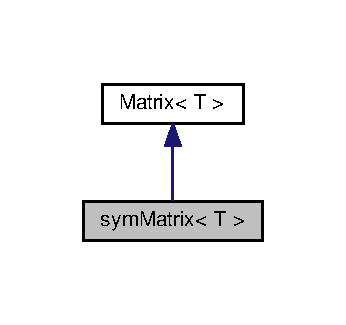
\includegraphics[width=166pt]{classsymMatrix__inherit__graph}
\end{center}
\end{figure}


Collaboration diagram for sym\+Matrix$<$ T $>$\+:\nopagebreak
\begin{figure}[H]
\begin{center}
\leavevmode
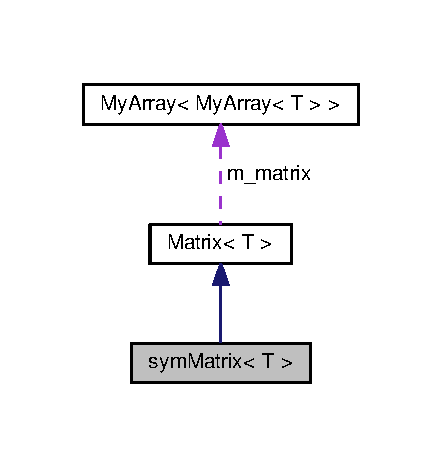
\includegraphics[width=212pt]{classsymMatrix__coll__graph}
\end{center}
\end{figure}
\subsection*{Public Member Functions}
\begin{DoxyCompactItemize}
\item 
\hyperlink{classsymMatrix_a7ccbe6ae7b25b2705fdf6fce29699d26}{sym\+Matrix} (const int size)
\item 
\hyperlink{classsymMatrix}{sym\+Matrix}$<$ T $>$ \& \hyperlink{classsymMatrix_ae2c26b03d13d63952f6052f88869b2e2}{operator=} (const \hyperlink{classsymMatrix}{sym\+Matrix}$<$ T $>$ \&rhs)
\item 
\hyperlink{classMatrix}{Matrix}$<$ T $>$ \hyperlink{classsymMatrix_a47071a21daf752e9a378c593ef85dbb2}{operator+} (const \hyperlink{classMatrix}{Matrix}$<$ T $>$ \&rhs) const 
\item 
\hyperlink{classMatrix}{Matrix}$<$ T $>$ \hyperlink{classsymMatrix_aaa418f9273ccc5da9d01c645e78ef657}{operator-\/} (const \hyperlink{classMatrix}{Matrix}$<$ T $>$ \&rhs) const 
\item 
\hyperlink{classMatrix}{Matrix}$<$ T $>$ \hyperlink{classsymMatrix_a4c1a9a20ab9bd68aca9f9d35d25e0e36}{operator$\ast$} (const \hyperlink{classMatrix}{Matrix}$<$ T $>$ \&rhs) const 
\item 
\hyperlink{classMyArray}{My\+Array}$<$ T $>$ \hyperlink{classsymMatrix_aa7adbc9378944126e08af6072ff648eb}{operator$\ast$} (const \hyperlink{classMyArray}{My\+Array}$<$ T $>$ \&rhs) const 
\item 
void \hyperlink{classsymMatrix_a75cb07e28a2ef936e45a7e3324429667}{scaler\+Multi} (const T scaler)
\item 
void \hyperlink{classsymMatrix_a06379c2668a6b1fba8b133d753a8f57c}{set\+Size} (const int size)
\item 
\hyperlink{classsymMatrix}{sym\+Matrix}$<$ T $>$ \hyperlink{classsymMatrix_aa3cfa46104ea3a5a6095ab20668a5445}{transpose} ()
\item 
void \hyperlink{classsymMatrix_a28d1f286c0a8572a26441afd635cba51}{set\+Matrix} (const int i, const int j, const T x)
\item 
T \hyperlink{classsymMatrix_a92bbf3194f8bf52559ee19ba706dd15c}{operator()} (const int i, const int j) const 
\item 
bool \hyperlink{classsymMatrix_a43d26e87d92d368544b9bd6384da8121}{is\+Diag\+Dom} () const 
\item 
void \hyperlink{classsymMatrix_adaa6f70fb421576d245f86c526b64ac1}{zero\+Me} ()
\end{DoxyCompactItemize}
\subsection*{Friends}
\begin{DoxyCompactItemize}
\item 
ostream \& \hyperlink{classsymMatrix_ab9fec73436f9148b1f7a85da84930bdf}{operator} (ostream \&out, const \hyperlink{classsymMatrix}{sym\+Matrix}$<$ T $>$ \&mat)
\item 
istream \& \hyperlink{classsymMatrix_a8a4d48a6277b6f343afee06fcb29ea53}{operator$>$$>$} (istream \&in, \hyperlink{classsymMatrix}{sym\+Matrix}$<$ T $>$ \&mat)
\end{DoxyCompactItemize}
\subsection*{Additional Inherited Members}


\subsection{Detailed Description}
\subsubsection*{template$<$class T$>$\\*
class sym\+Matrix$<$ T $>$}

\hyperlink{classsymMatrix}{sym\+Matrix} calss Reprents a NxN \hyperlink{classsymMatrix}{sym\+Matrix} \hyperlink{classMatrix}{Matrix} contains a\+: m\+\_\+size -\/ represting the size of N m\+\_\+matrix -\/ an my\+Array of my\+Arrays represting the matrix 

\subsection{Constructor \& Destructor Documentation}
\index{sym\+Matrix@{sym\+Matrix}!sym\+Matrix@{sym\+Matrix}}
\index{sym\+Matrix@{sym\+Matrix}!sym\+Matrix@{sym\+Matrix}}
\subsubsection[{\texorpdfstring{sym\+Matrix(const int size)}{symMatrix(const int size)}}]{\setlength{\rightskip}{0pt plus 5cm}template$<$typename T $>$ {\bf sym\+Matrix}$<$ T $>$\+::{\bf sym\+Matrix} (
\begin{DoxyParamCaption}
\item[{const int}]{size}
\end{DoxyParamCaption}
)}\hypertarget{classsymMatrix_a7ccbe6ae7b25b2705fdf6fce29699d26}{}\label{classsymMatrix_a7ccbe6ae7b25b2705fdf6fce29699d26}
initialize constructor. A new \hyperlink{classsymMatrix}{sym\+Matrix} is craeted with dimensions equel to \char`\"{}size\char`\"{} \begin{DoxyPrecond}{Precondition}
size must be bigger then 0! Will throw a a length Error otherwise 
\end{DoxyPrecond}
\begin{DoxyPostcond}{Postcondition}
a \hyperlink{classsymMatrix}{sym\+Matrix} is born! 
\end{DoxyPostcond}


\subsection{Member Function Documentation}
\index{sym\+Matrix@{sym\+Matrix}!is\+Diag\+Dom@{is\+Diag\+Dom}}
\index{is\+Diag\+Dom@{is\+Diag\+Dom}!sym\+Matrix@{sym\+Matrix}}
\subsubsection[{\texorpdfstring{is\+Diag\+Dom() const }{isDiagDom() const }}]{\setlength{\rightskip}{0pt plus 5cm}template$<$typename T $>$ bool {\bf sym\+Matrix}$<$ T $>$\+::is\+Diag\+Dom (
\begin{DoxyParamCaption}
{}
\end{DoxyParamCaption}
) const\hspace{0.3cm}{\ttfamily [virtual]}}\hypertarget{classsymMatrix_a43d26e87d92d368544b9bd6384da8121}{}\label{classsymMatrix_a43d26e87d92d368544b9bd6384da8121}
is diagonally dominant returns true if matrix is diagonally dominant. false otherwise. \begin{DoxyPrecond}{Precondition}
none 
\end{DoxyPrecond}
\begin{DoxyPostcond}{Postcondition}
none 
\end{DoxyPostcond}


Reimplemented from \hyperlink{classMatrix_ab5deedc9644d1b8c6bc220dd336f0102}{Matrix$<$ T $>$}.

\index{sym\+Matrix@{sym\+Matrix}!operator()@{operator()}}
\index{operator()@{operator()}!sym\+Matrix@{sym\+Matrix}}
\subsubsection[{\texorpdfstring{operator()(const int i, const int j) const }{operator()(const int i, const int j) const }}]{\setlength{\rightskip}{0pt plus 5cm}template$<$typename T $>$ T {\bf sym\+Matrix}$<$ T $>$\+::{\bf operator}() (
\begin{DoxyParamCaption}
\item[{const int}]{i, }
\item[{const int}]{j}
\end{DoxyParamCaption}
) const\hspace{0.3cm}{\ttfamily [virtual]}}\hypertarget{classsymMatrix_a92bbf3194f8bf52559ee19ba706dd15c}{}\label{classsymMatrix_a92bbf3194f8bf52559ee19ba706dd15c}
operaotr () returns value of m\+\_\+matrix\mbox{[}i\mbox{]}\mbox{[}j\mbox{]} \begin{DoxyPrecond}{Precondition}
0 $<$ i,j $<$size 
\end{DoxyPrecond}
\begin{DoxyPostcond}{Postcondition}
none 
\end{DoxyPostcond}


Reimplemented from \hyperlink{classMatrix_af786e95d49ae55d42c3bd6824a64e032}{Matrix$<$ T $>$}.

\index{sym\+Matrix@{sym\+Matrix}!operator$\ast$@{operator$\ast$}}
\index{operator$\ast$@{operator$\ast$}!sym\+Matrix@{sym\+Matrix}}
\subsubsection[{\texorpdfstring{operator$\ast$(const Matrix$<$ T $>$ \&rhs) const }{operator*(const Matrix< T > &rhs) const }}]{\setlength{\rightskip}{0pt plus 5cm}template$<$typename T $>$ {\bf Matrix}$<$ T $>$ {\bf sym\+Matrix}$<$ T $>$\+::{\bf operator}$\ast$ (
\begin{DoxyParamCaption}
\item[{const {\bf Matrix}$<$ T $>$ \&}]{rhs}
\end{DoxyParamCaption}
) const\hspace{0.3cm}{\ttfamily [virtual]}}\hypertarget{classsymMatrix_a4c1a9a20ab9bd68aca9f9d35d25e0e36}{}\label{classsymMatrix_a4c1a9a20ab9bd68aca9f9d35d25e0e36}
\hyperlink{classMatrix}{Matrix} multiplication caclualtes the multiplication of \hyperlink{classsymMatrix}{sym\+Matrix} and matrix, returens a new matrix with the calculated values \begin{DoxyPrecond}{Precondition}
size of CO must be equel to rhs, Will throw a a length Error otherwise. \char`\"{}$\ast$\char`\"{} binary operator must be defiend for T. 
\end{DoxyPrecond}
\begin{DoxyPostcond}{Postcondition}
a matrix is born! 
\end{DoxyPostcond}


Reimplemented from \hyperlink{classMatrix_a358516deb804403fb91256a5a269d1e2}{Matrix$<$ T $>$}.

\index{sym\+Matrix@{sym\+Matrix}!operator$\ast$@{operator$\ast$}}
\index{operator$\ast$@{operator$\ast$}!sym\+Matrix@{sym\+Matrix}}
\subsubsection[{\texorpdfstring{operator$\ast$(const My\+Array$<$ T $>$ \&rhs) const }{operator*(const MyArray< T > &rhs) const }}]{\setlength{\rightskip}{0pt plus 5cm}template$<$typename T $>$ {\bf My\+Array}$<$ T $>$ {\bf sym\+Matrix}$<$ T $>$\+::{\bf operator}$\ast$ (
\begin{DoxyParamCaption}
\item[{const {\bf My\+Array}$<$ T $>$ \&}]{rhs}
\end{DoxyParamCaption}
) const\hspace{0.3cm}{\ttfamily [virtual]}}\hypertarget{classsymMatrix_aa7adbc9378944126e08af6072ff648eb}{}\label{classsymMatrix_aa7adbc9378944126e08af6072ff648eb}
\hyperlink{classMatrix}{Matrix} -\/ Vector multiplication caclualtes the multiplication of a \hyperlink{classsymMatrix}{sym\+Matrix} with an Array and returens a new Vector with the calculated values \begin{DoxyPrecond}{Precondition}
size of CO must be equel to rhs array size! Will throw a a length Error otherwise. \char`\"{}$\ast$\char`\"{} binary operator must be defiend for T. 
\end{DoxyPrecond}
\begin{DoxyPostcond}{Postcondition}
a Vector is born! 
\end{DoxyPostcond}


Reimplemented from \hyperlink{classMatrix_a70c46247336f74291cc3e1b2fb800a34}{Matrix$<$ T $>$}.

\index{sym\+Matrix@{sym\+Matrix}!operator+@{operator+}}
\index{operator+@{operator+}!sym\+Matrix@{sym\+Matrix}}
\subsubsection[{\texorpdfstring{operator+(const Matrix$<$ T $>$ \&rhs) const }{operator+(const Matrix< T > &rhs) const }}]{\setlength{\rightskip}{0pt plus 5cm}template$<$typename T $>$ {\bf Matrix}$<$ T $>$ {\bf sym\+Matrix}$<$ T $>$\+::{\bf operator}+ (
\begin{DoxyParamCaption}
\item[{const {\bf Matrix}$<$ T $>$ \&}]{rhs}
\end{DoxyParamCaption}
) const\hspace{0.3cm}{\ttfamily [virtual]}}\hypertarget{classsymMatrix_a47071a21daf752e9a378c593ef85dbb2}{}\label{classsymMatrix_a47071a21daf752e9a378c593ef85dbb2}

\begin{DoxyItemize}
\item operator adds the sum of CO to rhs, retures a new \hyperlink{classMatrix}{Matrix} with the calculated values \begin{DoxyPrecond}{Precondition}
size of CO must be equel to rhs, Will throw a a length Error otherwise. \char`\"{}+\char`\"{} binary operator must be defiend for T. 
\end{DoxyPrecond}
\begin{DoxyPostcond}{Postcondition}
a matrix is born! 
\end{DoxyPostcond}

\end{DoxyItemize}

Reimplemented from \hyperlink{classMatrix_a9db4b4074daa2112eab910c7902fc5d9}{Matrix$<$ T $>$}.

\index{sym\+Matrix@{sym\+Matrix}!operator-\/@{operator-\/}}
\index{operator-\/@{operator-\/}!sym\+Matrix@{sym\+Matrix}}
\subsubsection[{\texorpdfstring{operator-\/(const Matrix$<$ T $>$ \&rhs) const }{operator-(const Matrix< T > &rhs) const }}]{\setlength{\rightskip}{0pt plus 5cm}template$<$typename T $>$ {\bf Matrix}$<$ T $>$ {\bf sym\+Matrix}$<$ T $>$\+::{\bf operator}-\/ (
\begin{DoxyParamCaption}
\item[{const {\bf Matrix}$<$ T $>$ \&}]{rhs}
\end{DoxyParamCaption}
) const\hspace{0.3cm}{\ttfamily [virtual]}}\hypertarget{classsymMatrix_aaa418f9273ccc5da9d01c645e78ef657}{}\label{classsymMatrix_aaa418f9273ccc5da9d01c645e78ef657}

\begin{DoxyItemize}
\item operator caclualtes the differnce of CO to rhs, retures a new \hyperlink{classMatrix}{Matrix} with the calculated values \begin{DoxyPrecond}{Precondition}
size of CO must be equel to rhs, Will throw a a length Error otherwise. \char`\"{}-\/\char`\"{} binary operator must be defiend for T. 
\end{DoxyPrecond}
\begin{DoxyPostcond}{Postcondition}
a matrix is born! 
\end{DoxyPostcond}

\end{DoxyItemize}

Reimplemented from \hyperlink{classMatrix_a06a7f018ed353f0a8239a80ec8403be6}{Matrix$<$ T $>$}.

\index{sym\+Matrix@{sym\+Matrix}!operator=@{operator=}}
\index{operator=@{operator=}!sym\+Matrix@{sym\+Matrix}}
\subsubsection[{\texorpdfstring{operator=(const sym\+Matrix$<$ T $>$ \&rhs)}{operator=(const symMatrix< T > &rhs)}}]{\setlength{\rightskip}{0pt plus 5cm}template$<$typename T $>$ {\bf sym\+Matrix}$<$ T $>$ \& {\bf sym\+Matrix}$<$ T $>$\+::{\bf operator}= (
\begin{DoxyParamCaption}
\item[{const {\bf sym\+Matrix}$<$ T $>$ \&}]{rhs}
\end{DoxyParamCaption}
)}\hypertarget{classsymMatrix_ae2c26b03d13d63952f6052f88869b2e2}{}\label{classsymMatrix_ae2c26b03d13d63952f6052f88869b2e2}
= assignment turns the CO \hyperlink{classsymMatrix}{sym\+Matrix} into R\+HS \hyperlink{classsymMatrix}{sym\+Matrix} \begin{DoxyPrecond}{Precondition}
none 
\end{DoxyPrecond}
\begin{DoxyPostcond}{Postcondition}
none 
\end{DoxyPostcond}
\index{sym\+Matrix@{sym\+Matrix}!scaler\+Multi@{scaler\+Multi}}
\index{scaler\+Multi@{scaler\+Multi}!sym\+Matrix@{sym\+Matrix}}
\subsubsection[{\texorpdfstring{scaler\+Multi(const T scaler)}{scalerMulti(const T scaler)}}]{\setlength{\rightskip}{0pt plus 5cm}template$<$typename T $>$ void {\bf sym\+Matrix}$<$ T $>$\+::scaler\+Multi (
\begin{DoxyParamCaption}
\item[{const T}]{scaler}
\end{DoxyParamCaption}
)\hspace{0.3cm}{\ttfamily [virtual]}}\hypertarget{classsymMatrix_a75cb07e28a2ef936e45a7e3324429667}{}\label{classsymMatrix_a75cb07e28a2ef936e45a7e3324429667}
\hyperlink{classMatrix}{Matrix} Scaler multiplication caclualtes the multiplication of a \hyperlink{classsymMatrix}{sym\+Matrix} with a scaler and modifies the CO m\+\_\+matrix with calculation \begin{DoxyPrecond}{Precondition}
\char`\"{}$\ast$\char`\"{} binary operator must be defiend for T. 
\end{DoxyPrecond}
\begin{DoxyPostcond}{Postcondition}
none 
\end{DoxyPostcond}


Reimplemented from \hyperlink{classMatrix_aba8c673e5ca3bcc56a9bad1a1c0fed23}{Matrix$<$ T $>$}.

\index{sym\+Matrix@{sym\+Matrix}!set\+Matrix@{set\+Matrix}}
\index{set\+Matrix@{set\+Matrix}!sym\+Matrix@{sym\+Matrix}}
\subsubsection[{\texorpdfstring{set\+Matrix(const int i, const int j, const T x)}{setMatrix(const int i, const int j, const T x)}}]{\setlength{\rightskip}{0pt plus 5cm}template$<$typename T $>$ void {\bf sym\+Matrix}$<$ T $>$\+::set\+Matrix (
\begin{DoxyParamCaption}
\item[{const int}]{i, }
\item[{const int}]{j, }
\item[{const T}]{x}
\end{DoxyParamCaption}
)\hspace{0.3cm}{\ttfamily [virtual]}}\hypertarget{classsymMatrix_a28d1f286c0a8572a26441afd635cba51}{}\label{classsymMatrix_a28d1f286c0a8572a26441afd635cba51}
Set \hyperlink{classMatrix}{Matrix} changes the value of m\+\_\+matrix\mbox{[}i\mbox{]}\mbox{[}j\mbox{]} and m\+\_\+matrix\mbox{[}j\mbox{]}\mbox{[}i\mbox{]} to x \begin{DoxyPrecond}{Precondition}
0 $<$ i,j $<$size 
\end{DoxyPrecond}
\begin{DoxyPostcond}{Postcondition}
modified m\+\_\+matrix 
\end{DoxyPostcond}


Reimplemented from \hyperlink{classMatrix_a0cf31a462707441cbbab037190c88f33}{Matrix$<$ T $>$}.

\index{sym\+Matrix@{sym\+Matrix}!set\+Size@{set\+Size}}
\index{set\+Size@{set\+Size}!sym\+Matrix@{sym\+Matrix}}
\subsubsection[{\texorpdfstring{set\+Size(const int size)}{setSize(const int size)}}]{\setlength{\rightskip}{0pt plus 5cm}template$<$typename T $>$ void {\bf sym\+Matrix}$<$ T $>$\+::set\+Size (
\begin{DoxyParamCaption}
\item[{const int}]{size}
\end{DoxyParamCaption}
)\hspace{0.3cm}{\ttfamily [virtual]}}\hypertarget{classsymMatrix_a06379c2668a6b1fba8b133d753a8f57c}{}\label{classsymMatrix_a06379c2668a6b1fba8b133d753a8f57c}
set size!

\begin{DoxyPrecond}{Precondition}
s must be postive 
\end{DoxyPrecond}
\begin{DoxyPostcond}{Postcondition}
none 
\end{DoxyPostcond}


Reimplemented from \hyperlink{classMatrix_a1add3e066eaaa19d5056fc6e2cbc767c}{Matrix$<$ T $>$}.

\index{sym\+Matrix@{sym\+Matrix}!transpose@{transpose}}
\index{transpose@{transpose}!sym\+Matrix@{sym\+Matrix}}
\subsubsection[{\texorpdfstring{transpose()}{transpose()}}]{\setlength{\rightskip}{0pt plus 5cm}template$<$typename T $>$ {\bf sym\+Matrix}$<$ T $>$ {\bf sym\+Matrix}$<$ T $>$\+::transpose (
\begin{DoxyParamCaption}
{}
\end{DoxyParamCaption}
)}\hypertarget{classsymMatrix_aa3cfa46104ea3a5a6095ab20668a5445}{}\label{classsymMatrix_aa3cfa46104ea3a5a6095ab20668a5445}
\hyperlink{classMatrix}{Matrix} transpose calculator Creates a new matrix with is a trasposed version of the CO \begin{DoxyPrecond}{Precondition}
none 
\end{DoxyPrecond}
\begin{DoxyPostcond}{Postcondition}
a \hyperlink{classMatrix}{Matrix} is born 
\end{DoxyPostcond}
\index{sym\+Matrix@{sym\+Matrix}!zero\+Me@{zero\+Me}}
\index{zero\+Me@{zero\+Me}!sym\+Matrix@{sym\+Matrix}}
\subsubsection[{\texorpdfstring{zero\+Me()}{zeroMe()}}]{\setlength{\rightskip}{0pt plus 5cm}template$<$typename T $>$ void {\bf sym\+Matrix}$<$ T $>$\+::zero\+Me (
\begin{DoxyParamCaption}
{}
\end{DoxyParamCaption}
)}\hypertarget{classsymMatrix_adaa6f70fb421576d245f86c526b64ac1}{}\label{classsymMatrix_adaa6f70fb421576d245f86c526b64ac1}
zero\+Me fills the matrix with the zero value \begin{DoxyPrecond}{Precondition}
none 
\end{DoxyPrecond}
\begin{DoxyPostcond}{Postcondition}
m\+\_\+matrix is modified 
\end{DoxyPostcond}


\subsection{Friends And Related Function Documentation}
\index{sym\+Matrix@{sym\+Matrix}!operator@{operator}}
\index{operator@{operator}!sym\+Matrix@{sym\+Matrix}}
\subsubsection[{\texorpdfstring{operator}{operator}}]{\setlength{\rightskip}{0pt plus 5cm}template$<$class T$>$ ostream\& operator (
\begin{DoxyParamCaption}
\item[{ostream \&}]{out, }
\item[{const {\bf sym\+Matrix}$<$ T $>$ \&}]{mat}
\end{DoxyParamCaption}
)\hspace{0.3cm}{\ttfamily [friend]}}\hypertarget{classsymMatrix_ab9fec73436f9148b1f7a85da84930bdf}{}\label{classsymMatrix_ab9fec73436f9148b1f7a85da84930bdf}
Stream insertion operator for {\ttfamily \hyperlink{classsymMatrix}{sym\+Matrix}}.

\begin{DoxyPrecond}{Precondition}
Stream insertion operator is defined for {\ttfamily T}. 
\end{DoxyPrecond}
\begin{DoxyPostcond}{Postcondition}
The contents of the m\+\_\+matrix are printed to the ouptut stream. Each array is printed on a new row. 
\end{DoxyPostcond}
\begin{DoxyReturn}{Returns}
the modified output stream. 
\end{DoxyReturn}
\index{sym\+Matrix@{sym\+Matrix}!operator$>$$>$@{operator$>$$>$}}
\index{operator$>$$>$@{operator$>$$>$}!sym\+Matrix@{sym\+Matrix}}
\subsubsection[{\texorpdfstring{operator$>$$>$}{operator>>}}]{\setlength{\rightskip}{0pt plus 5cm}template$<$class T$>$ istream\& {\bf operator}$>$$>$ (
\begin{DoxyParamCaption}
\item[{istream \&}]{in, }
\item[{{\bf sym\+Matrix}$<$ T $>$ \&}]{mat}
\end{DoxyParamCaption}
)\hspace{0.3cm}{\ttfamily [friend]}}\hypertarget{classsymMatrix_a8a4d48a6277b6f343afee06fcb29ea53}{}\label{classsymMatrix_a8a4d48a6277b6f343afee06fcb29ea53}
Stream insertion operator for {\ttfamily \hyperlink{classsymMatrix}{sym\+Matrix}}.

\begin{DoxyPrecond}{Precondition}
Stream insertion operator is defined for {\ttfamily T}. 
\end{DoxyPrecond}
\begin{DoxyPostcond}{Postcondition}
the m\+\_\+matrix if filled with the input 
\end{DoxyPostcond}
\begin{DoxyReturn}{Returns}
the modified input stream. 
\end{DoxyReturn}


The documentation for this class was generated from the following files\+:\begin{DoxyCompactItemize}
\item 
\hyperlink{symMatrix_8h}{sym\+Matrix.\+h}\item 
sym\+Matrix.\+hpp\end{DoxyCompactItemize}

\chapter{File Documentation}
\hypertarget{deepdec_8h}{}\section{deepdec.\+h File Reference}
\label{deepdec_8h}\index{deepdec.\+h@{deepdec.\+h}}
{\ttfamily \#include \char`\"{}my\+Array.\+h\char`\"{}}\\*
{\ttfamily \#include \char`\"{}sym\+Matrix.\+h\char`\"{}}\\*
{\ttfamily \#include $<$stdexcept$>$}\\*
{\ttfamily \#include $<$cmath$>$}\\*
{\ttfamily \#include \char`\"{}deepdec.\+hpp\char`\"{}}\\*
Include dependency graph for deepdec.\+h\+:\nopagebreak
\begin{figure}[H]
\begin{center}
\leavevmode
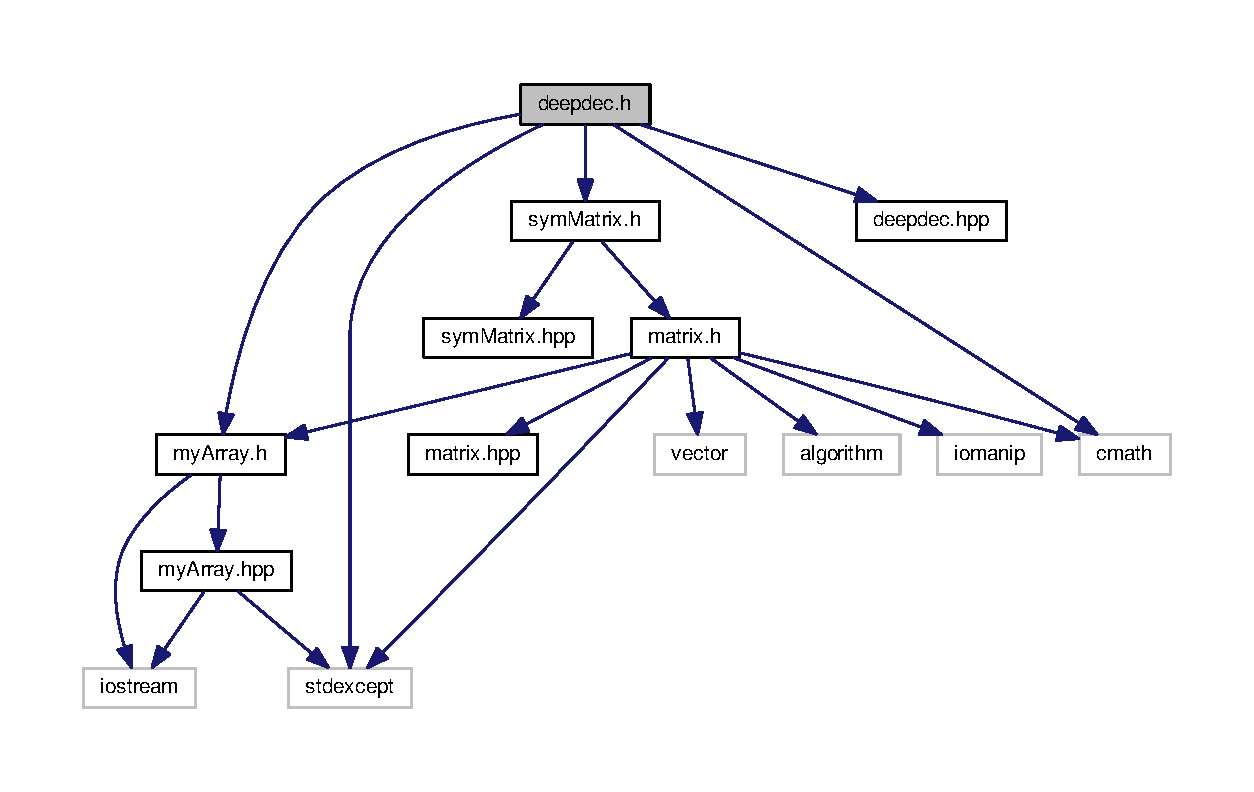
\includegraphics[width=350pt]{deepdec_8h__incl}
\end{center}
\end{figure}
\subsection*{Classes}
\begin{DoxyCompactItemize}
\item 
class \hyperlink{classdeepDec}{deep\+Dec$<$ T $>$}
\end{DoxyCompactItemize}


\subsection{Detailed Description}
the steepest descent class 
\hypertarget{gauss__seidel_8h}{}\section{gauss\+\_\+seidel.\+h File Reference}
\label{gauss__seidel_8h}\index{gauss\+\_\+seidel.\+h@{gauss\+\_\+seidel.\+h}}
{\ttfamily \#include \char`\"{}my\+Array.\+h\char`\"{}}\\*
{\ttfamily \#include \char`\"{}sym\+Matrix.\+h\char`\"{}}\\*
{\ttfamily \#include $<$stdexcept$>$}\\*
{\ttfamily \#include $<$cmath$>$}\\*
{\ttfamily \#include \char`\"{}gauss\+\_\+seidel.\+hpp\char`\"{}}\\*
Include dependency graph for gauss\+\_\+seidel.\+h\+:\nopagebreak
\begin{figure}[H]
\begin{center}
\leavevmode
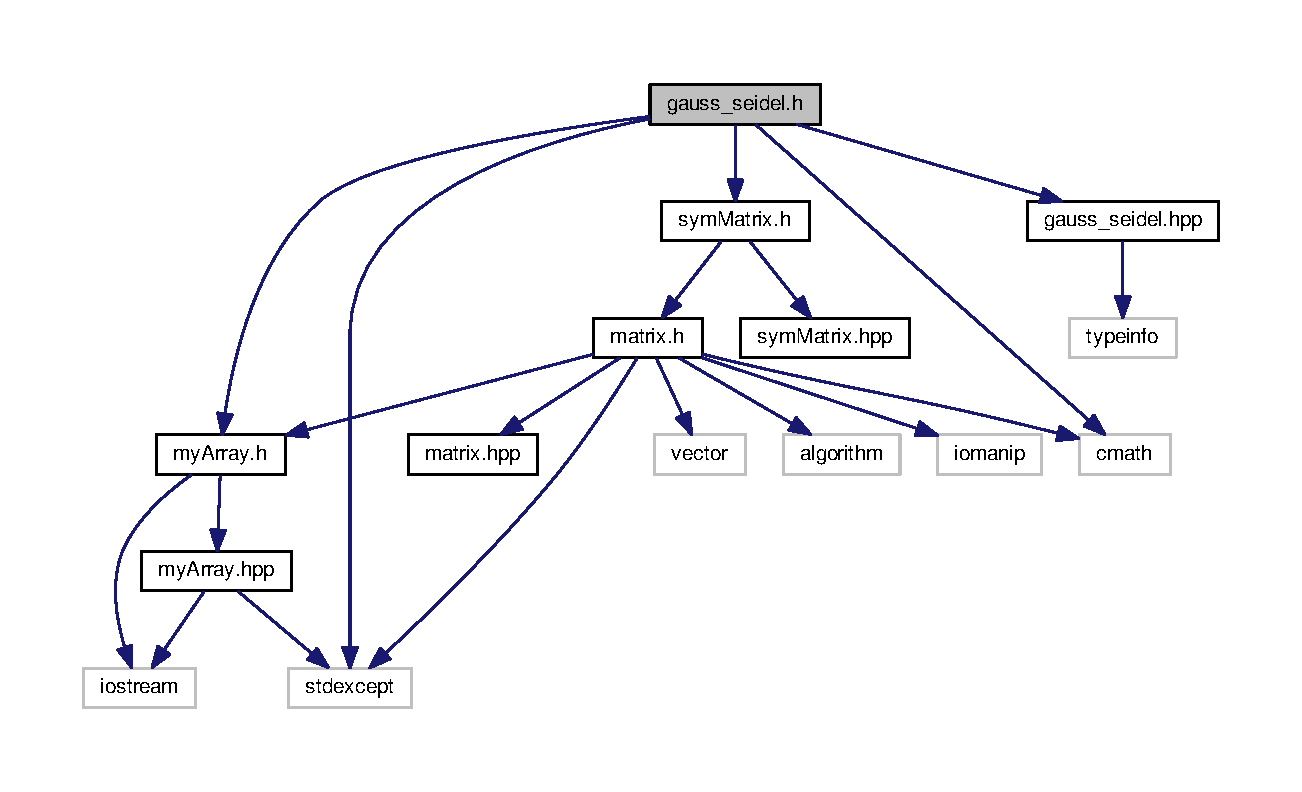
\includegraphics[width=350pt]{gauss__seidel_8h__incl}
\end{center}
\end{figure}
\subsection*{Classes}
\begin{DoxyCompactItemize}
\item 
class \hyperlink{classgauss__seidel}{gauss\+\_\+seidel$<$ T $>$}
\end{DoxyCompactItemize}


\subsection{Detailed Description}
the Gauss-\/\+Seidel class. 
\hypertarget{matrix_8h}{}\section{matrix.\+h File Reference}
\label{matrix_8h}\index{matrix.\+h@{matrix.\+h}}
{\ttfamily \#include \char`\"{}my\+Array.\+h\char`\"{}}\\*
{\ttfamily \#include $<$vector$>$}\\*
{\ttfamily \#include $<$algorithm$>$}\\*
{\ttfamily \#include $<$cmath$>$}\\*
{\ttfamily \#include $<$iomanip$>$}\\*
{\ttfamily \#include $<$stdexcept$>$}\\*
{\ttfamily \#include \char`\"{}matrix.\+hpp\char`\"{}}\\*
Include dependency graph for matrix.\+h\+:\nopagebreak
\begin{figure}[H]
\begin{center}
\leavevmode
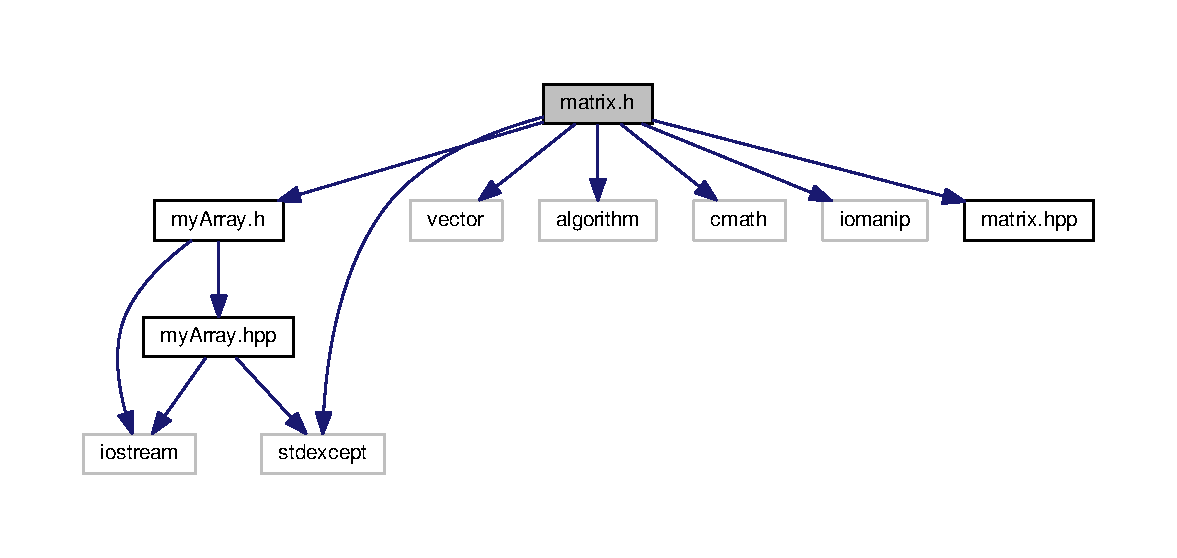
\includegraphics[width=350pt]{matrix_8h__incl}
\end{center}
\end{figure}
This graph shows which files directly or indirectly include this file\+:\nopagebreak
\begin{figure}[H]
\begin{center}
\leavevmode
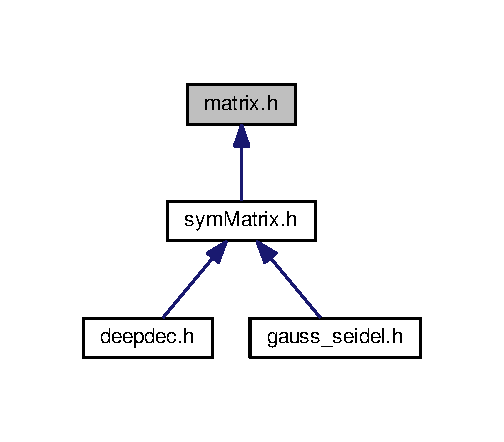
\includegraphics[width=242pt]{matrix_8h__dep__incl}
\end{center}
\end{figure}
\subsection*{Classes}
\begin{DoxyCompactItemize}
\item 
class \hyperlink{classMatrix}{Matrix$<$ T $>$}
\item 
class \hyperlink{classMatrix}{Matrix$<$ T $>$}
\item 
class \hyperlink{classCompare}{Compare$<$ T $>$}
\end{DoxyCompactItemize}
\subsection*{Functions}
\begin{DoxyCompactItemize}
\item 
{\footnotesize template$<$class T $>$ }\\ostream \& \hyperlink{matrix_8h_aabfdf243bf6d7e452fcef8553c128096}{operator$<$$<$} (ostream \&out, \hyperlink{classMatrix}{Matrix}$<$ T $>$ \&mat)
\item 
{\footnotesize template$<$class T $>$ }\\istream \& \hyperlink{matrix_8h_a9a32964bf1d2e4e86dd2d34bc310bdcf}{operator$>$$>$} (istream \&in, \hyperlink{classMatrix}{Matrix}$<$ T $>$ \&mat)
\end{DoxyCompactItemize}


\subsection{Detailed Description}
A \hyperlink{classMatrix}{Matrix} class. 

\subsection{Function Documentation}
\index{matrix.\+h@{matrix.\+h}!operator$<$$<$@{operator$<$$<$}}
\index{operator$<$$<$@{operator$<$$<$}!matrix.\+h@{matrix.\+h}}
\subsubsection[{\texorpdfstring{operator$<$$<$(ostream \&out, Matrix$<$ T $>$ \&mat)}{operator<<(ostream &out, Matrix< T > &mat)}}]{\setlength{\rightskip}{0pt plus 5cm}template$<$class T $>$ ostream\& operator$<$$<$ (
\begin{DoxyParamCaption}
\item[{ostream \&}]{out, }
\item[{{\bf Matrix}$<$ T $>$ \&}]{mat}
\end{DoxyParamCaption}
)}\hypertarget{matrix_8h_aabfdf243bf6d7e452fcef8553c128096}{}\label{matrix_8h_aabfdf243bf6d7e452fcef8553c128096}
Stream insertion operator for {\ttfamily \hyperlink{classMatrix}{Matrix}}.

\begin{DoxyPrecond}{Precondition}
Stream insertion operator is defined for {\ttfamily T}. 
\end{DoxyPrecond}
\begin{DoxyPostcond}{Postcondition}
The contents of the m\+\_\+matrix are printed to the ouptut stream. Each array is printed on a new row. 
\end{DoxyPostcond}
\begin{DoxyReturn}{Returns}
the modified output stream. 
\end{DoxyReturn}
\index{matrix.\+h@{matrix.\+h}!operator$>$$>$@{operator$>$$>$}}
\index{operator$>$$>$@{operator$>$$>$}!matrix.\+h@{matrix.\+h}}
\subsubsection[{\texorpdfstring{operator$>$$>$(istream \&in, Matrix$<$ T $>$ \&mat)}{operator>>(istream &in, Matrix< T > &mat)}}]{\setlength{\rightskip}{0pt plus 5cm}template$<$class T $>$ istream\& operator$>$$>$ (
\begin{DoxyParamCaption}
\item[{istream \&}]{in, }
\item[{{\bf Matrix}$<$ T $>$ \&}]{mat}
\end{DoxyParamCaption}
)}\hypertarget{matrix_8h_a9a32964bf1d2e4e86dd2d34bc310bdcf}{}\label{matrix_8h_a9a32964bf1d2e4e86dd2d34bc310bdcf}
Stream insertion operator for {\ttfamily \hyperlink{classMatrix}{Matrix}}.

\begin{DoxyPrecond}{Precondition}
Stream insertion operator is defined for {\ttfamily T}. 
\end{DoxyPrecond}
\begin{DoxyPostcond}{Postcondition}
the m\+\_\+matrix if filled with the input 
\end{DoxyPostcond}
\begin{DoxyReturn}{Returns}
the modified input stream. 
\end{DoxyReturn}

\hypertarget{mesh_8h}{}\section{mesh.\+h File Reference}
\label{mesh_8h}\index{mesh.\+h@{mesh.\+h}}
{\ttfamily \#include $<$iostream$>$}\\*
{\ttfamily \#include \char`\"{}mesh.\+hpp\char`\"{}}\\*
Include dependency graph for mesh.\+h\+:\nopagebreak
\begin{figure}[H]
\begin{center}
\leavevmode
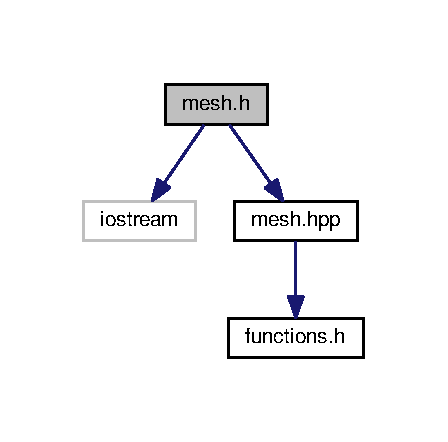
\includegraphics[width=215pt]{mesh_8h__incl}
\end{center}
\end{figure}
\subsection*{Classes}
\begin{DoxyCompactItemize}
\item 
class \hyperlink{classmesh}{mesh$<$ T $>$}
\end{DoxyCompactItemize}


\subsection{Detailed Description}
the Mesh class. 
\hypertarget{myArray_8h}{}\section{my\+Array.\+h File Reference}
\label{myArray_8h}\index{my\+Array.\+h@{my\+Array.\+h}}
{\ttfamily \#include $<$iostream$>$}\\*
{\ttfamily \#include \char`\"{}my\+Array.\+hpp\char`\"{}}\\*
Include dependency graph for my\+Array.\+h\+:\nopagebreak
\begin{figure}[H]
\begin{center}
\leavevmode
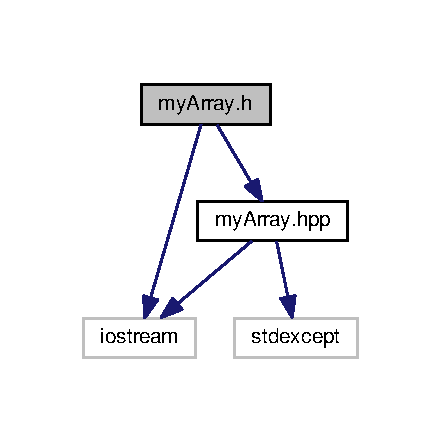
\includegraphics[width=212pt]{myArray_8h__incl}
\end{center}
\end{figure}
This graph shows which files directly or indirectly include this file\+:\nopagebreak
\begin{figure}[H]
\begin{center}
\leavevmode
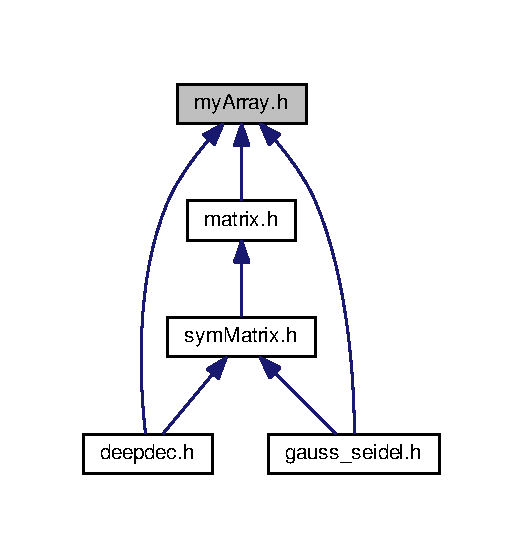
\includegraphics[width=251pt]{myArray_8h__dep__incl}
\end{center}
\end{figure}
\subsection*{Classes}
\begin{DoxyCompactItemize}
\item 
class \hyperlink{classMyArray}{My\+Array$<$ T $>$}
\item 
class \hyperlink{classMyArray}{My\+Array$<$ T $>$}
\end{DoxyCompactItemize}
\subsection*{Functions}
\begin{DoxyCompactItemize}
\item 
{\footnotesize template$<$class T $>$ }\\ostream \& \hyperlink{myArray_8h_a19bba46c1d0e61a60716e519dce35694}{operator$<$$<$} (ostream \&out, const \hyperlink{classMyArray}{My\+Array}$<$ T $>$ \&arr)
\end{DoxyCompactItemize}


\subsection{Detailed Description}
An Array class. 

\subsection{Function Documentation}
\index{my\+Array.\+h@{my\+Array.\+h}!operator$<$$<$@{operator$<$$<$}}
\index{operator$<$$<$@{operator$<$$<$}!my\+Array.\+h@{my\+Array.\+h}}
\subsubsection[{\texorpdfstring{operator$<$$<$(ostream \&out, const My\+Array$<$ T $>$ \&arr)}{operator<<(ostream &out, const MyArray< T > &arr)}}]{\setlength{\rightskip}{0pt plus 5cm}template$<$class T $>$ ostream\& operator$<$$<$ (
\begin{DoxyParamCaption}
\item[{ostream \&}]{out, }
\item[{const {\bf My\+Array}$<$ T $>$ \&}]{arr}
\end{DoxyParamCaption}
)}\hypertarget{myArray_8h_a19bba46c1d0e61a60716e519dce35694}{}\label{myArray_8h_a19bba46c1d0e61a60716e519dce35694}
Stream insertion operator for {\ttfamily my\+Array}.

\begin{DoxyPrecond}{Precondition}
Stream insertion operator is defined for {\ttfamily T}. 
\end{DoxyPrecond}
\begin{DoxyPostcond}{Postcondition}
The contents of the interval\+Data are printed to the ouptut stream. 
\end{DoxyPostcond}
\begin{DoxyReturn}{Returns}
the modified output stream. 
\end{DoxyReturn}

\hypertarget{symMatrix_8h}{}\section{sym\+Matrix.\+h File Reference}
\label{symMatrix_8h}\index{sym\+Matrix.\+h@{sym\+Matrix.\+h}}
{\ttfamily \#include \char`\"{}matrix.\+h\char`\"{}}\\*
{\ttfamily \#include \char`\"{}sym\+Matrix.\+hpp\char`\"{}}\\*
Include dependency graph for sym\+Matrix.\+h\+:\nopagebreak
\begin{figure}[H]
\begin{center}
\leavevmode
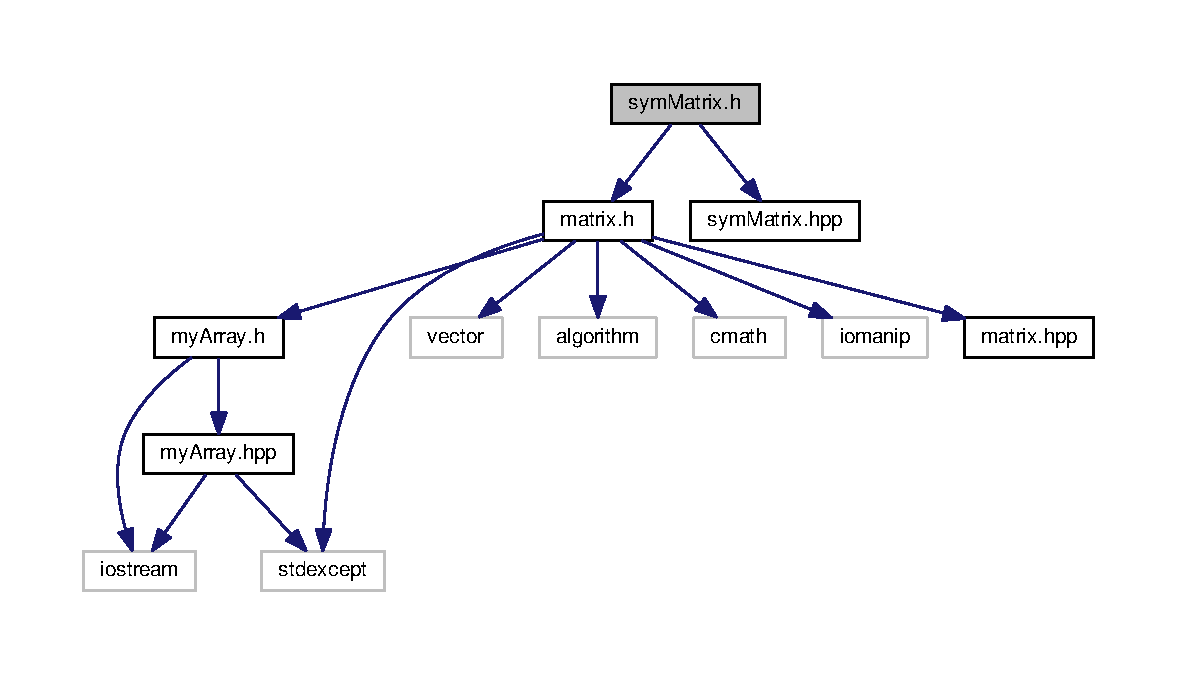
\includegraphics[width=350pt]{symMatrix_8h__incl}
\end{center}
\end{figure}
This graph shows which files directly or indirectly include this file\+:\nopagebreak
\begin{figure}[H]
\begin{center}
\leavevmode
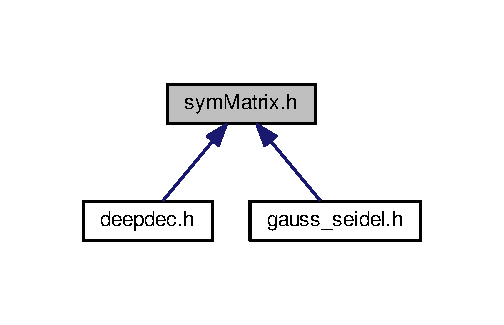
\includegraphics[width=242pt]{symMatrix_8h__dep__incl}
\end{center}
\end{figure}
\subsection*{Classes}
\begin{DoxyCompactItemize}
\item 
class \hyperlink{classsymMatrix}{sym\+Matrix$<$ T $>$}
\item 
class \hyperlink{classsymMatrix}{sym\+Matrix$<$ T $>$}
\end{DoxyCompactItemize}
\subsection*{Functions}
\begin{DoxyCompactItemize}
\item 
{\footnotesize template$<$class T $>$ }\\ostream \& \hyperlink{symMatrix_8h_a47c6313276439b28a6fa0473ab7cd798}{operator$<$$<$} (ostream \&out, const \hyperlink{classsymMatrix}{sym\+Matrix}$<$ T $>$ \&mat)
\item 
{\footnotesize template$<$class T $>$ }\\istream \& \hyperlink{symMatrix_8h_a17cb2fcfa986c7c501dc2fcc28c421db}{operator$>$$>$} (istream \&in, \hyperlink{classsymMatrix}{sym\+Matrix}$<$ T $>$ \&mat)
\end{DoxyCompactItemize}


\subsection{Detailed Description}
the symmatric matrix class 

\subsection{Function Documentation}
\index{sym\+Matrix.\+h@{sym\+Matrix.\+h}!operator$<$$<$@{operator$<$$<$}}
\index{operator$<$$<$@{operator$<$$<$}!sym\+Matrix.\+h@{sym\+Matrix.\+h}}
\subsubsection[{\texorpdfstring{operator$<$$<$(ostream \&out, const sym\+Matrix$<$ T $>$ \&mat)}{operator<<(ostream &out, const symMatrix< T > &mat)}}]{\setlength{\rightskip}{0pt plus 5cm}template$<$class T $>$ ostream\& operator$<$$<$ (
\begin{DoxyParamCaption}
\item[{ostream \&}]{out, }
\item[{const {\bf sym\+Matrix}$<$ T $>$ \&}]{mat}
\end{DoxyParamCaption}
)}\hypertarget{symMatrix_8h_a47c6313276439b28a6fa0473ab7cd798}{}\label{symMatrix_8h_a47c6313276439b28a6fa0473ab7cd798}
Stream insertion operator for {\ttfamily \hyperlink{classsymMatrix}{sym\+Matrix}}.

\begin{DoxyPrecond}{Precondition}
Stream insertion operator is defined for {\ttfamily T}. 
\end{DoxyPrecond}
\begin{DoxyPostcond}{Postcondition}
The contents of the m\+\_\+matrix are printed to the ouptut stream. Each array is printed on a new row. 
\end{DoxyPostcond}
\begin{DoxyReturn}{Returns}
the modified output stream. 
\end{DoxyReturn}
\index{sym\+Matrix.\+h@{sym\+Matrix.\+h}!operator$>$$>$@{operator$>$$>$}}
\index{operator$>$$>$@{operator$>$$>$}!sym\+Matrix.\+h@{sym\+Matrix.\+h}}
\subsubsection[{\texorpdfstring{operator$>$$>$(istream \&in, sym\+Matrix$<$ T $>$ \&mat)}{operator>>(istream &in, symMatrix< T > &mat)}}]{\setlength{\rightskip}{0pt plus 5cm}template$<$class T $>$ istream\& operator$>$$>$ (
\begin{DoxyParamCaption}
\item[{istream \&}]{in, }
\item[{{\bf sym\+Matrix}$<$ T $>$ \&}]{mat}
\end{DoxyParamCaption}
)}\hypertarget{symMatrix_8h_a17cb2fcfa986c7c501dc2fcc28c421db}{}\label{symMatrix_8h_a17cb2fcfa986c7c501dc2fcc28c421db}
Stream insertion operator for {\ttfamily \hyperlink{classsymMatrix}{sym\+Matrix}}.

\begin{DoxyPrecond}{Precondition}
Stream insertion operator is defined for {\ttfamily T}. 
\end{DoxyPrecond}
\begin{DoxyPostcond}{Postcondition}
the m\+\_\+matrix if filled with the input 
\end{DoxyPostcond}
\begin{DoxyReturn}{Returns}
the modified input stream. 
\end{DoxyReturn}

%--- End generated contents ---

% Index
\backmatter
\newpage
\phantomsection
\clearemptydoublepage
\addcontentsline{toc}{chapter}{Index}
\printindex

\end{document}
